%%==================================================
%% chapter04.tex for TJU Master Thesis
%% Encoding: UTF-8
%%==================================================

\chapter{基于峰值频移目标函数的反射全波形反演}

论文第三章提出的$Q$-RWI框架是基于数据残差的最小二乘目标函数来实现的,该目标泛函
对于理论的合成数据有很理想的效果,那是因为在合成数据实验中我们假设已知了模型
速度的高波数成分和低波数成分,即振幅的残差只由$Q$不准引起。
在实际勘探地震数据处理中,要获取低波数的速度模型相对可行,高波数的速度
模型很难精确获取,而高波数的速度成分又是影响地震波振幅的最大因素。此外,
地震波振幅还受数据采集环境的影响,如环境噪音、检波器与地表耦合情况等。
引起振幅残差的成因的不确定性给第三章提出的基于数据残差最小的$Q$-RWI法造成了致命
的影响。

如何孤立地将地震衰减对地震数据的影响从数据中提取出来是$Q$-RWI法走向实用的关键。
本章将从地震数据属性出发,寻找只与$Q$相关的地震数据属性,
并将其应用到$Q$-RWI中。

\vspace{1.0cm}
\section{引言}
\begin{figure*}[!htbp]
    \centering
    \subfigure[]{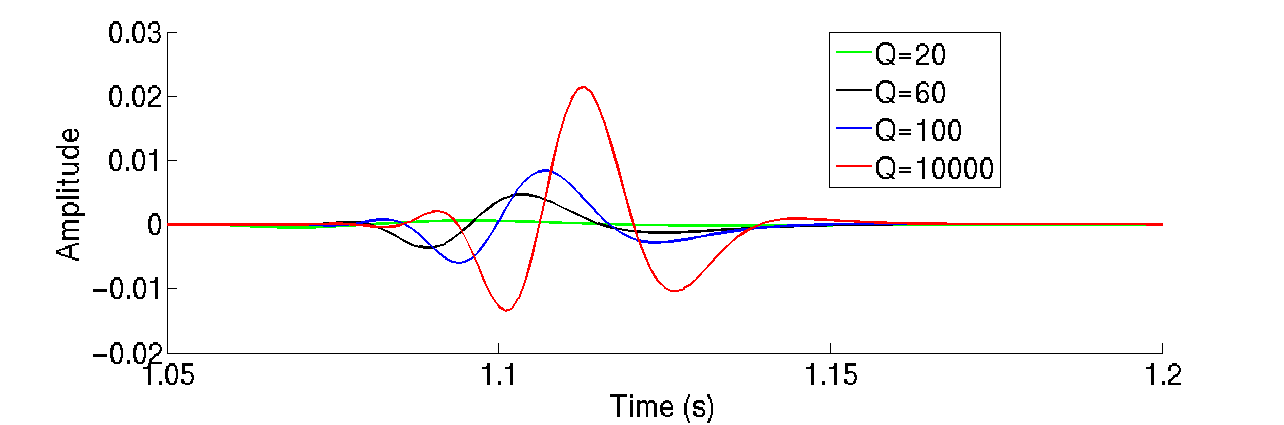
\includegraphics[width=0.92\linewidth]{figure/wavelet}}
    \subfigure[]{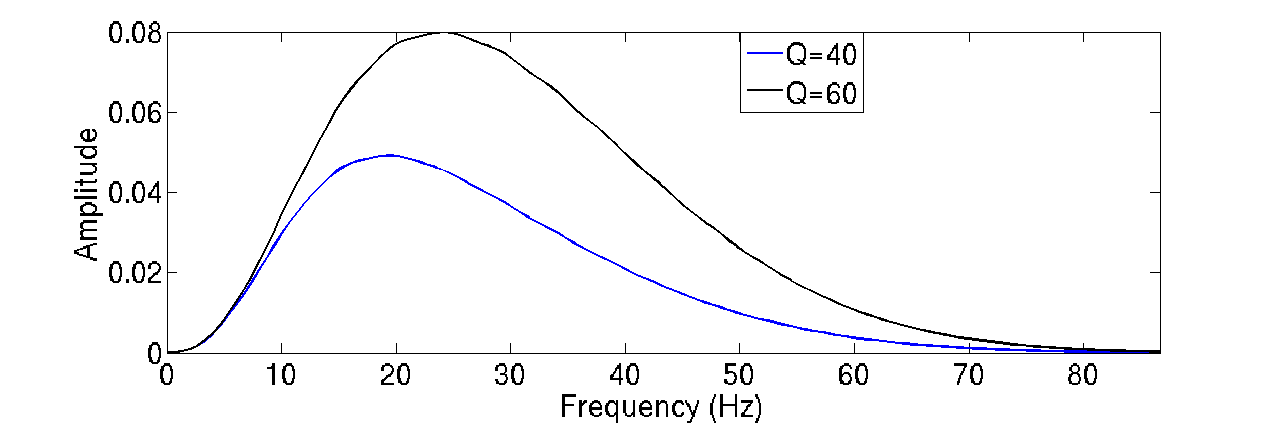
\includegraphics[width=0.92\linewidth]{figure/spectrum}}
    \subfigure[]{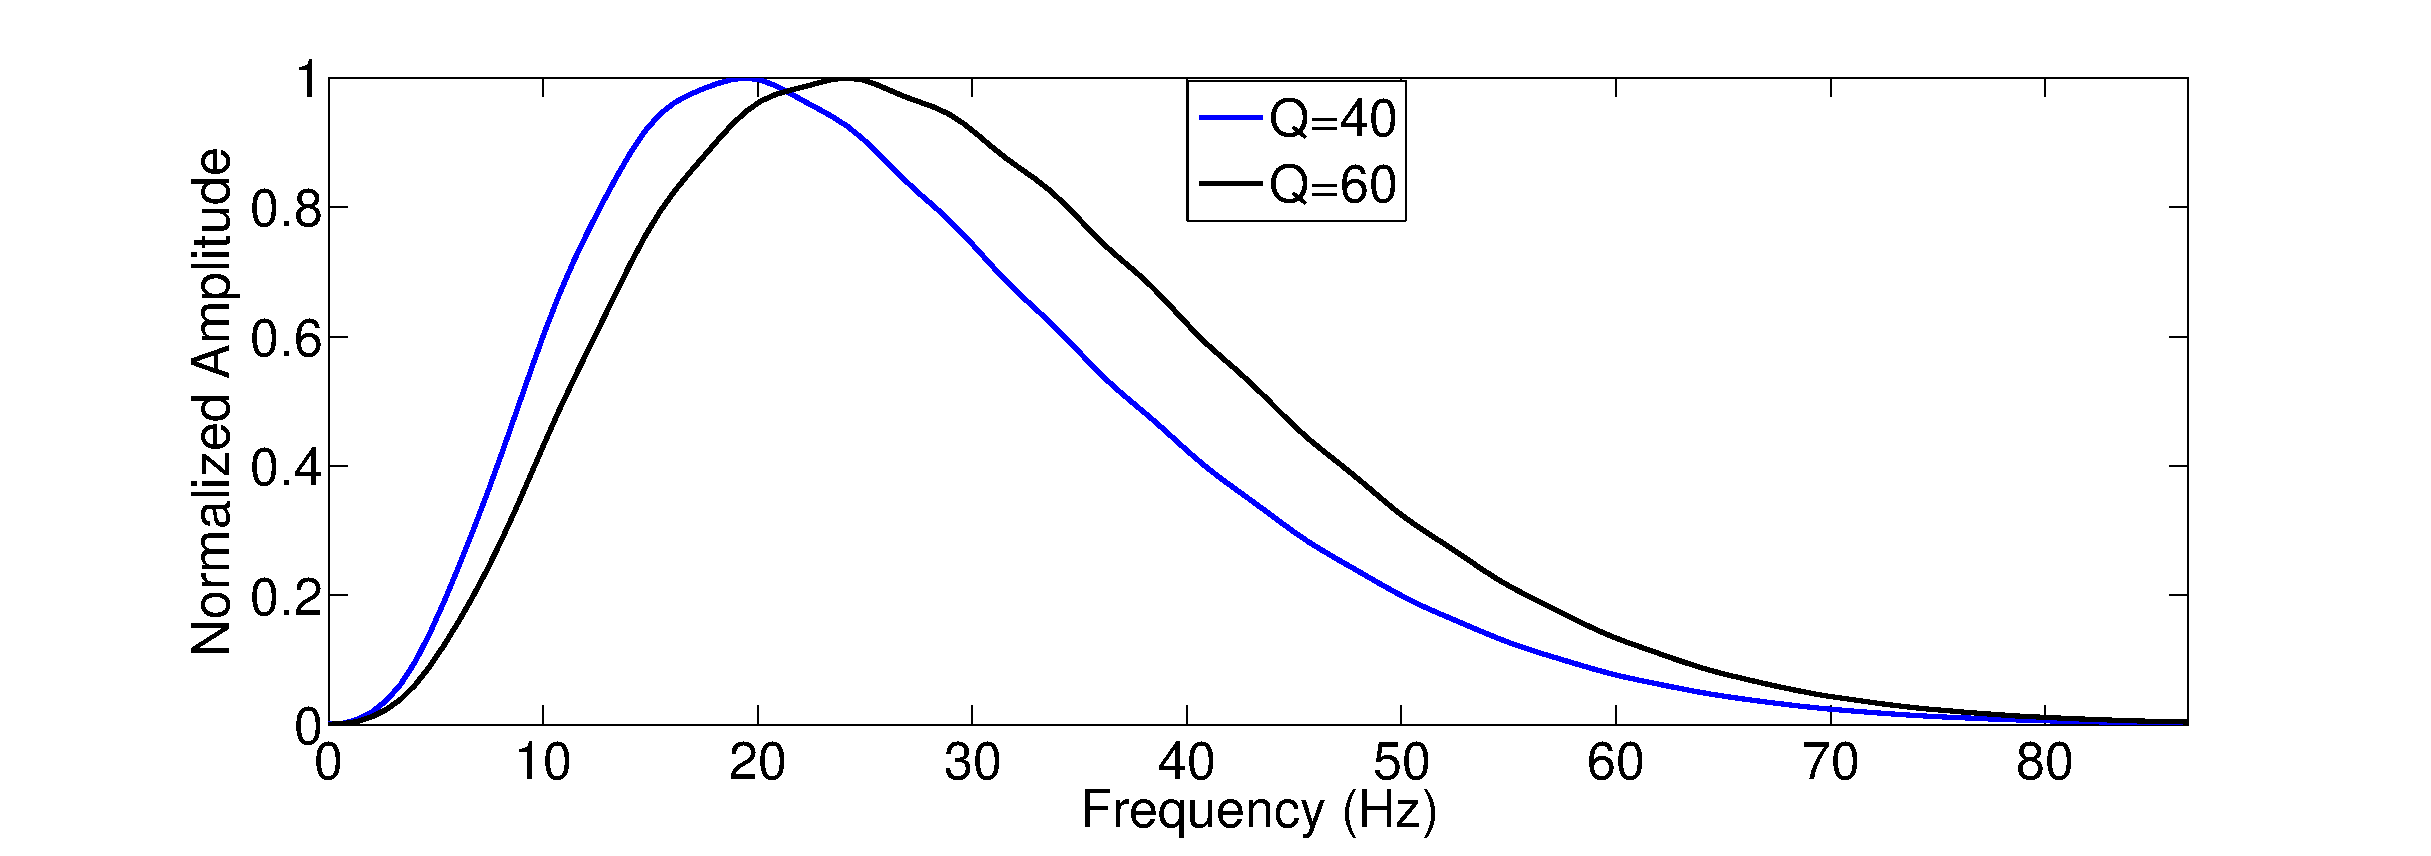
\includegraphics[width=0.92\linewidth]{figure/normalized_spectrum}}
    \fcaption{地震衰减效应:(a)不同$Q$值对地震波波形的影响;(b)不同$Q$值对地震波
	振幅谱的影响;(c)归一化的振幅谱。}{The effects of seismic attenuation:
    (a) the seismic waveforms propagated in different $Q$ models; (b) the amplitude 
	spectrum; (c) the nomalized amplitude spectrum.}
    [地震衰减效应]
    \label{fig:q_effect}
\end{figure*}
地震衰减不仅吸收地震波的振幅而且对地震波的相位有很强的改造作用(图~\ref{fig:q_effect}a)。
由第二章的线性粘弹理论知道,衰减系数$\alpha$与地震波的频率$f$成线性关系
(公式~\ref{eq:linear_visco}),即$\alpha\propto f$。
衰减介质对地震波高频成分的衰减要强于对低频成分的衰减(图~\ref{fig:q_effect}b),
这就导致了衰减介质中地震波的峰值频率往低频率处移动(图~\ref{fig:q_effect}c)。
几何扩散、透射损失等地震现象影响地震波的振幅但不影响地震波的峰值频率,
地震波峰值频率的大小基本只与地下介质衰减强度有关。\citeB{quan.harris:1997}
首次将模拟数据与观测数据间的质心频率差异作为匹配准则,用射线层析方程来更新
$Q$模型。为了克服射线理论高频近似的局限性,\citeB{dutta.schuster:2016}将峰值
频率移动目标函数引入到了波动层析当中,通过链接函数首次推导了压力波场对
驰豫参数$\tau(\mathbf{x})$的Frechet导数。同时也用伴随状态法推导出了峰值频率移动目标
函数对模型参数$\tau(\mathbf{x})$的梯度并给出了伴随源。他们的方法在理论合成数据
和实际数据中都获得了很好的效果,但是\citeB{dutta.schuster:2016}的$Q$层析方法
只用了直达波数据。

\begin{figure*}[!htbp]
    \centering
    {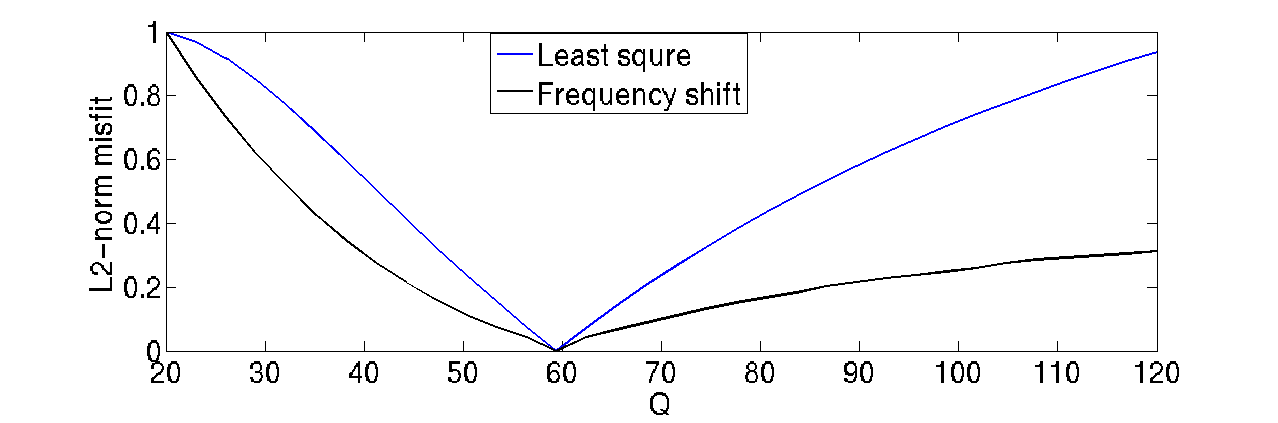
\includegraphics[width=0.92\linewidth]{figure/misfit_com}}
    \fcaption{两类归一化的目标函数随$Q$变化的形态,蓝线表示数据残差匹配最小二乘目
	标泛函,黑线表示峰值频率移动最小二乘目标泛函。}
	{Two types of misfit function vary with $Q$, blue line represents the least 
	squre of amplitue residual, and the black line represents the least squre of 
	the frequency shift.}[两类归一化的目标函数随$Q$变化的形态]
    \label{fig:misfit_com}
\end{figure*}
正如第三章所讲,相较于透射波,反射波能提供更深部的介质参数信息。
相比于振幅匹配的目标函数(公式~\ref{eq:misfit_function}),峰值频率移动的
目标函数具有如下表达式:
\begin{equation}
    \mathcal{J}(\mathbf{m})=\frac{1}{2}\sum_{s,g}\int_t\Delta f^2(\mathbf{x}_s,\mathbf{x}_g,t)dt,
    \label{eq:freq_misfit_function}
\end{equation}
其中$\Delta f(\mathbf{x}_s,\mathbf{x}_g,t)=f^{peak}_{obs}(\mathbf{x}_s,\mathbf{x}_g,t)-
f^{peak}_{cal}(\mathbf{x}_s,\mathbf{x}_g,t)$,$f^{peak}_{obs}(\mathbf{x}_s,\mathbf{x}_g,t)$
和$f^{peak}_{cal}(\mathbf{x}_s,\mathbf{x}_g,t)$分别是观测数据与模拟数据各震相的峰值
频率。图~\ref{fig:misfit_com}~展示了两种目标函数随$Q$值变化的形态。从图中可以看出
峰值频率移动的目标函数比波形残差目标函数具有更宽的收敛盆,更加适合背景$Q$模型的反演。

另外,将峰值频率移动作为匹配准则引入$Q$-RWI中可以降低反演方法对高波数速度模型的依赖。
图~\ref{fig:smooth_model}将两层速度模型通过平滑获得了平滑半径为16的低波数背景模型以及
不同平滑尺度的高波数扰动模型。其对应的地震波模拟结果如图~\ref{fig:smooth}所示,其中
红线是用粘声波方程模拟的结果,其余均为Born正演结果,从图中可以看出Born正演对高波数速度
的平滑尺度不敏感,同样其振幅谱也不敏感。当固定上层速度为2100m/s,下层速度从1700m/s变化
到3500m/s时,Born正演(用相同的平滑半径来分解高低波数速度成分)的地震数据
(图~\ref{fig:contrast}a)虽具有不同的振幅,
地震数据的极性也可能发生变化,但从归一化的振幅谱
(图~\ref{fig:contrast}c)中可以看出其地震数据具有相同的峰值频率。
在Born正演中,峰值频率对高波数速度模型的结构、大小以及极性均不敏感,因此
用峰值频率移动作为测量准则极大的降低了$Q$-RWI对高波数速度成分的依赖性。

反射波数据不同于直达波数据,通常具有多个震相。如何把反射波数据中各个震相的
峰值频率提取出来是反演成功的关键。本章先介绍基于峰值频率移动目标函数的
$Q$-RWI基本理论;然后给出提取多震相反射地震数据各个震相峰值频率的办法;
最后通过数值实验来证明所提反演方法的可靠性。

\begin{figure*}[!htbp]
    \centering
    \subfigure[]{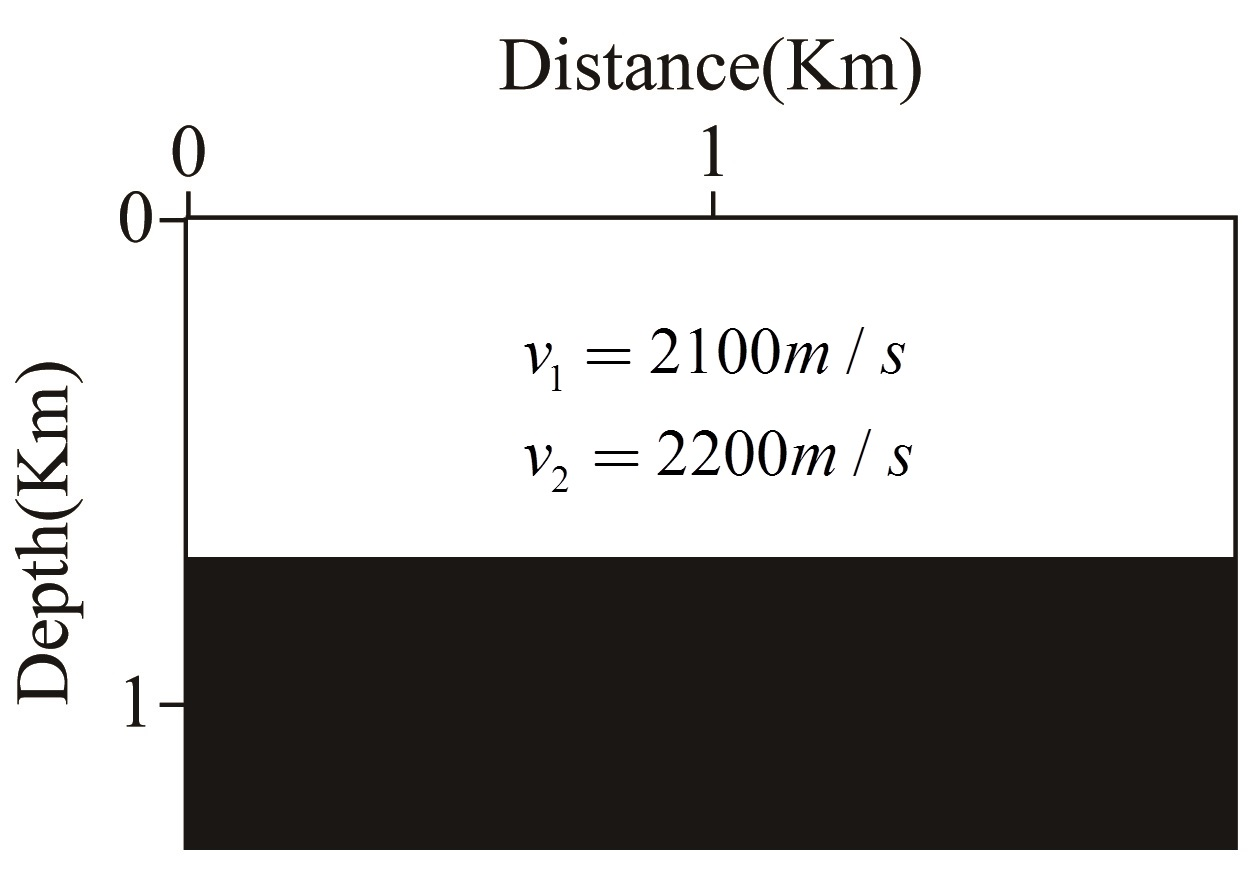
\includegraphics[width=0.32\linewidth]{figure/modelv}}
    \subfigure[]{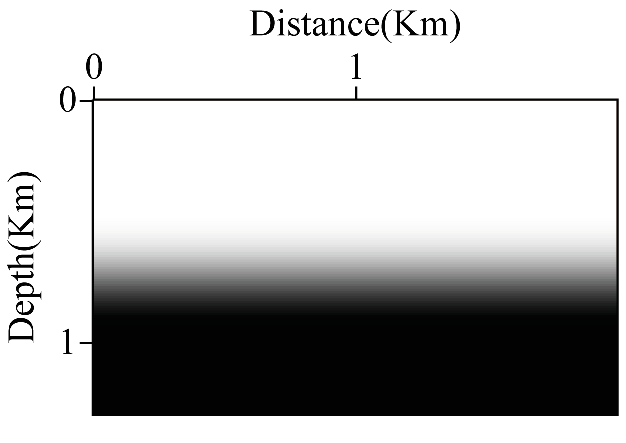
\includegraphics[width=0.32\linewidth]{figure/modelv0}}
    \subfigure[]{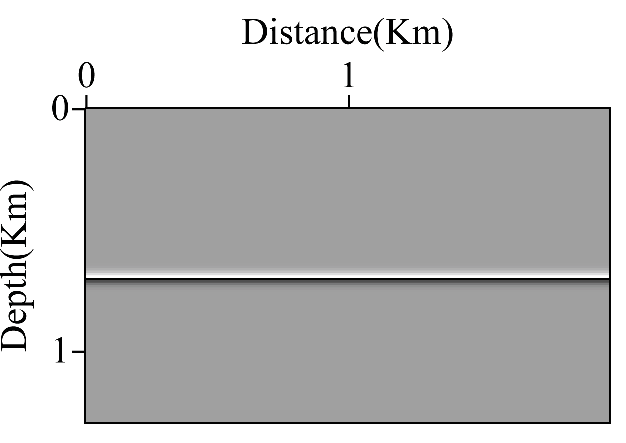
\includegraphics[width=0.32\linewidth]{figure/dvel_s4}}
    \subfigure[]{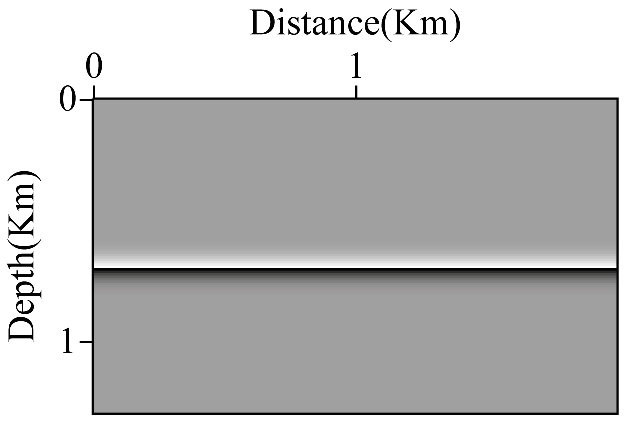
\includegraphics[width=0.32\linewidth]{figure/dvel_s8}}
    \subfigure[]{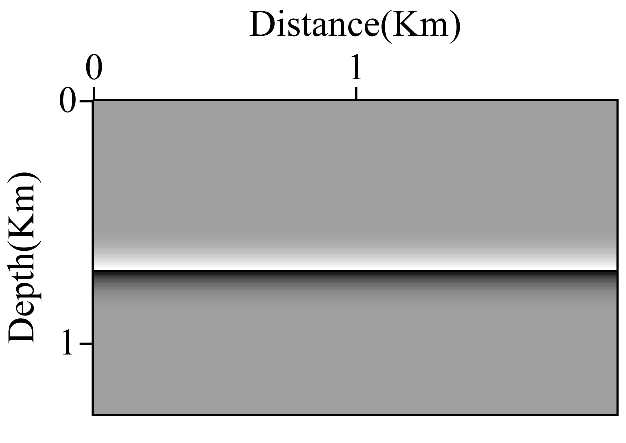
\includegraphics[width=0.32\linewidth]{figure/dvel_s12}}
    \subfigure[]{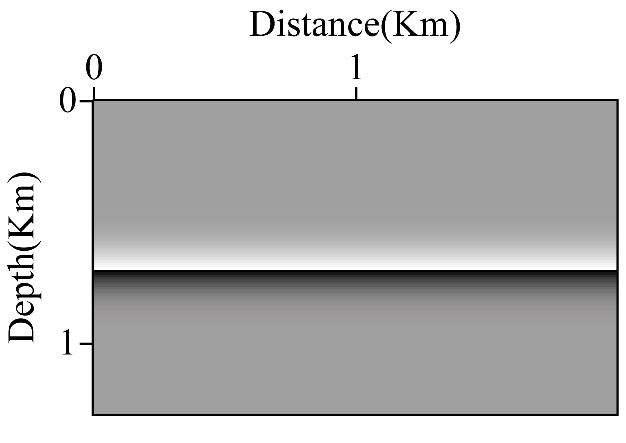
\includegraphics[width=0.32\linewidth]{figure/dvel_s16}}
    \fcaption{Born正演的不同平滑尺度速度模型分解:(a)真实两层速度模型;(b)平滑半径为16
	的光滑背景速度;(c)平滑半径为4的高波数速度;(d)平滑半径为8的高波数速度;
	(e)平滑半径为12的高波数速度;(f)平滑半径为16的高波数速度。}{Different smooth scales 
	decomposition of velocity for Born modeling: (a) the two-layer velocity model; 
	(b) the background velocity with 12 smooth radius; (c) the perturbation velocity with 
	4 smooth radius; (d) the perturbation velocity with 8 smooth radius; (e) the perturbation 
	velocity with 12 smooth radius; (f) the perturbation velocity with 16 smooth radius.}
    [Born正演的不同平滑尺度速度模型分解]
    \label{fig:smooth_model}
\end{figure*}

\begin{figure*}[!htbp]
    \centering
    \subfigure[]{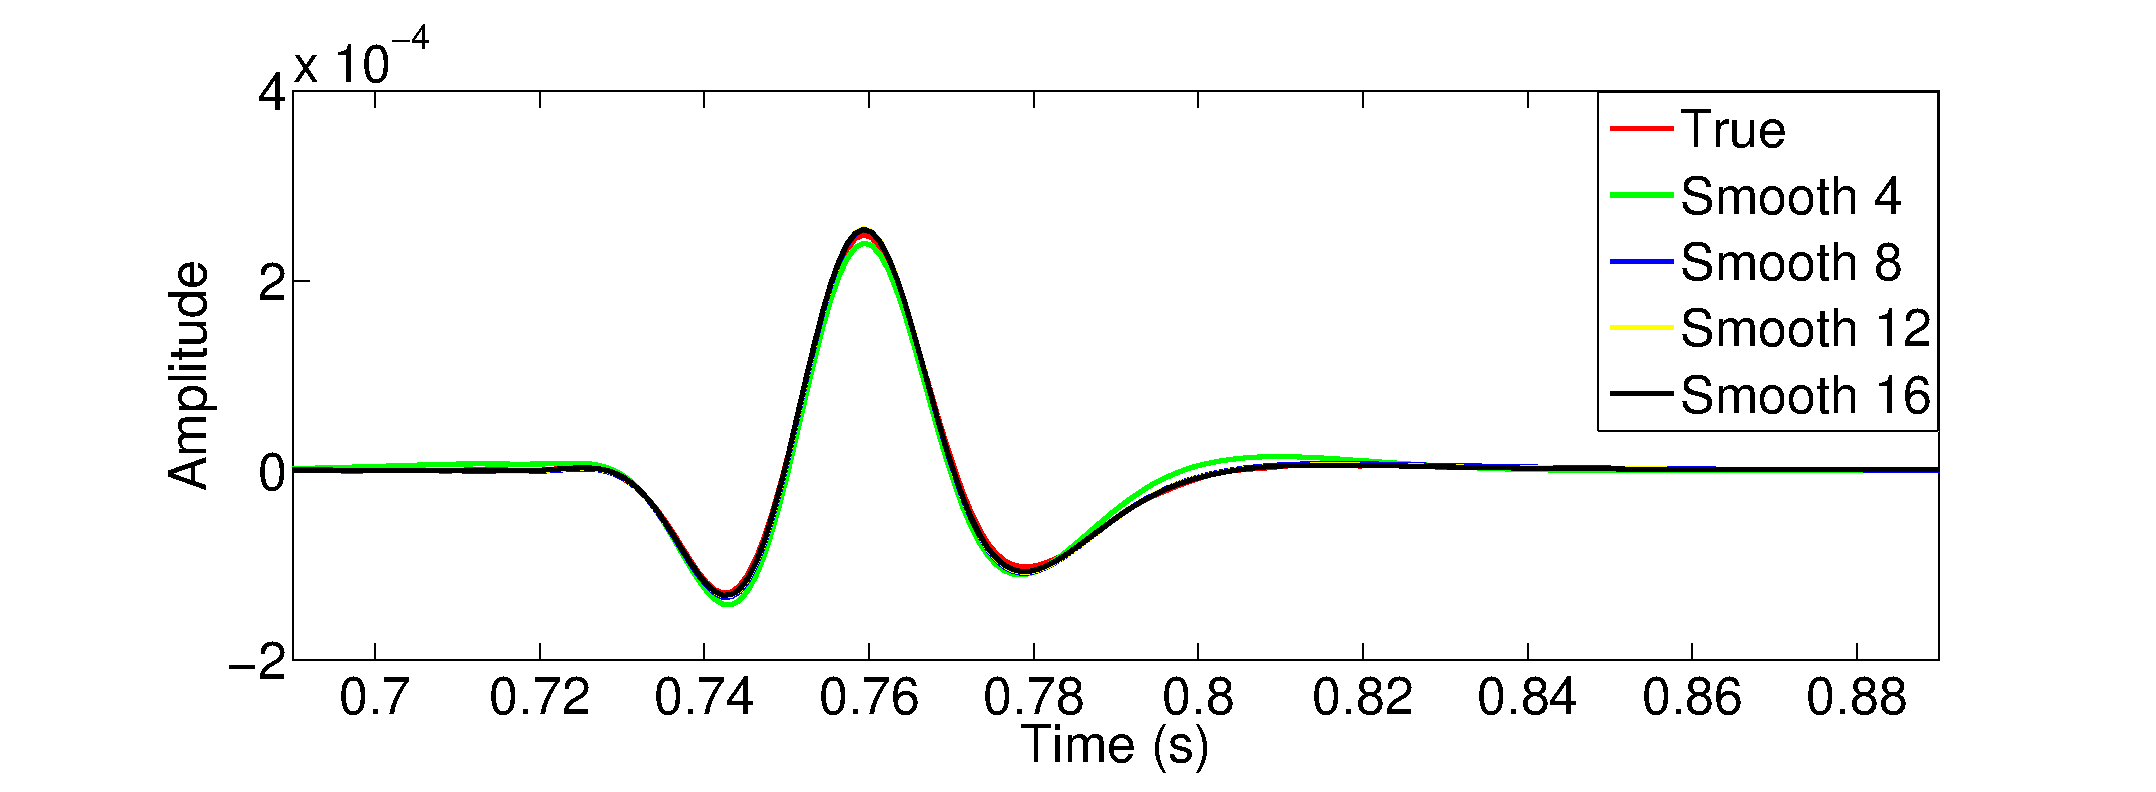
\includegraphics[width=0.92\linewidth]{figure/traces_ch4}}
    \subfigure[]{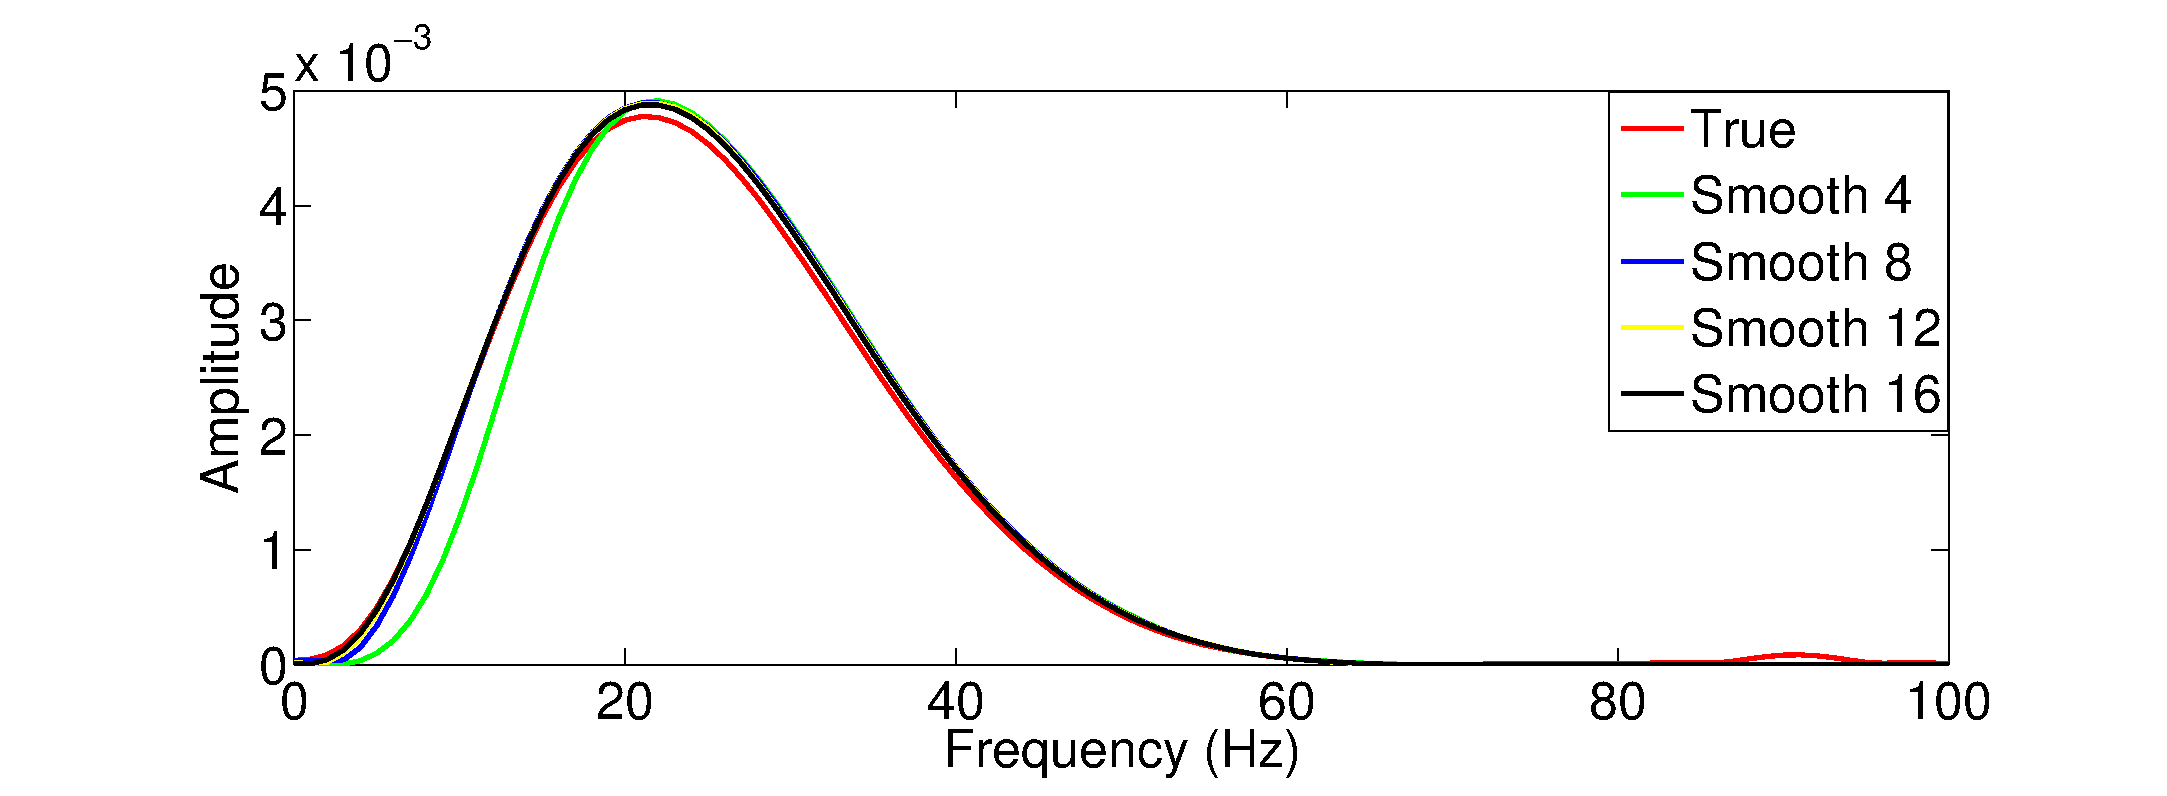
\includegraphics[width=0.92\linewidth]{figure/spectral_ch4}}
	\fcaption{不同平滑尺度速度模型分解的Born正演地震响应:(a)对应于\ref{fig:smooth_model}
	的地震响应,其中红线是用粘声波方程模拟的结果,其余是用不同平滑尺度分解出的高波数速度Born
	正演的结果;(b)对应地震数据的振幅谱。}{Born modeling results for different velcity 
	perturbations: (a) seismic response corresponding Figure~\ref{fig:smooth_model}; 
	(b) the amplitude spectral for the seismic traces.}
    [不同平滑尺度速度模型分解的Born正演地震响应]
    \label{fig:smooth}
\end{figure*}

\begin{figure*}[!htbp]
    \centering
    \subfigure[]{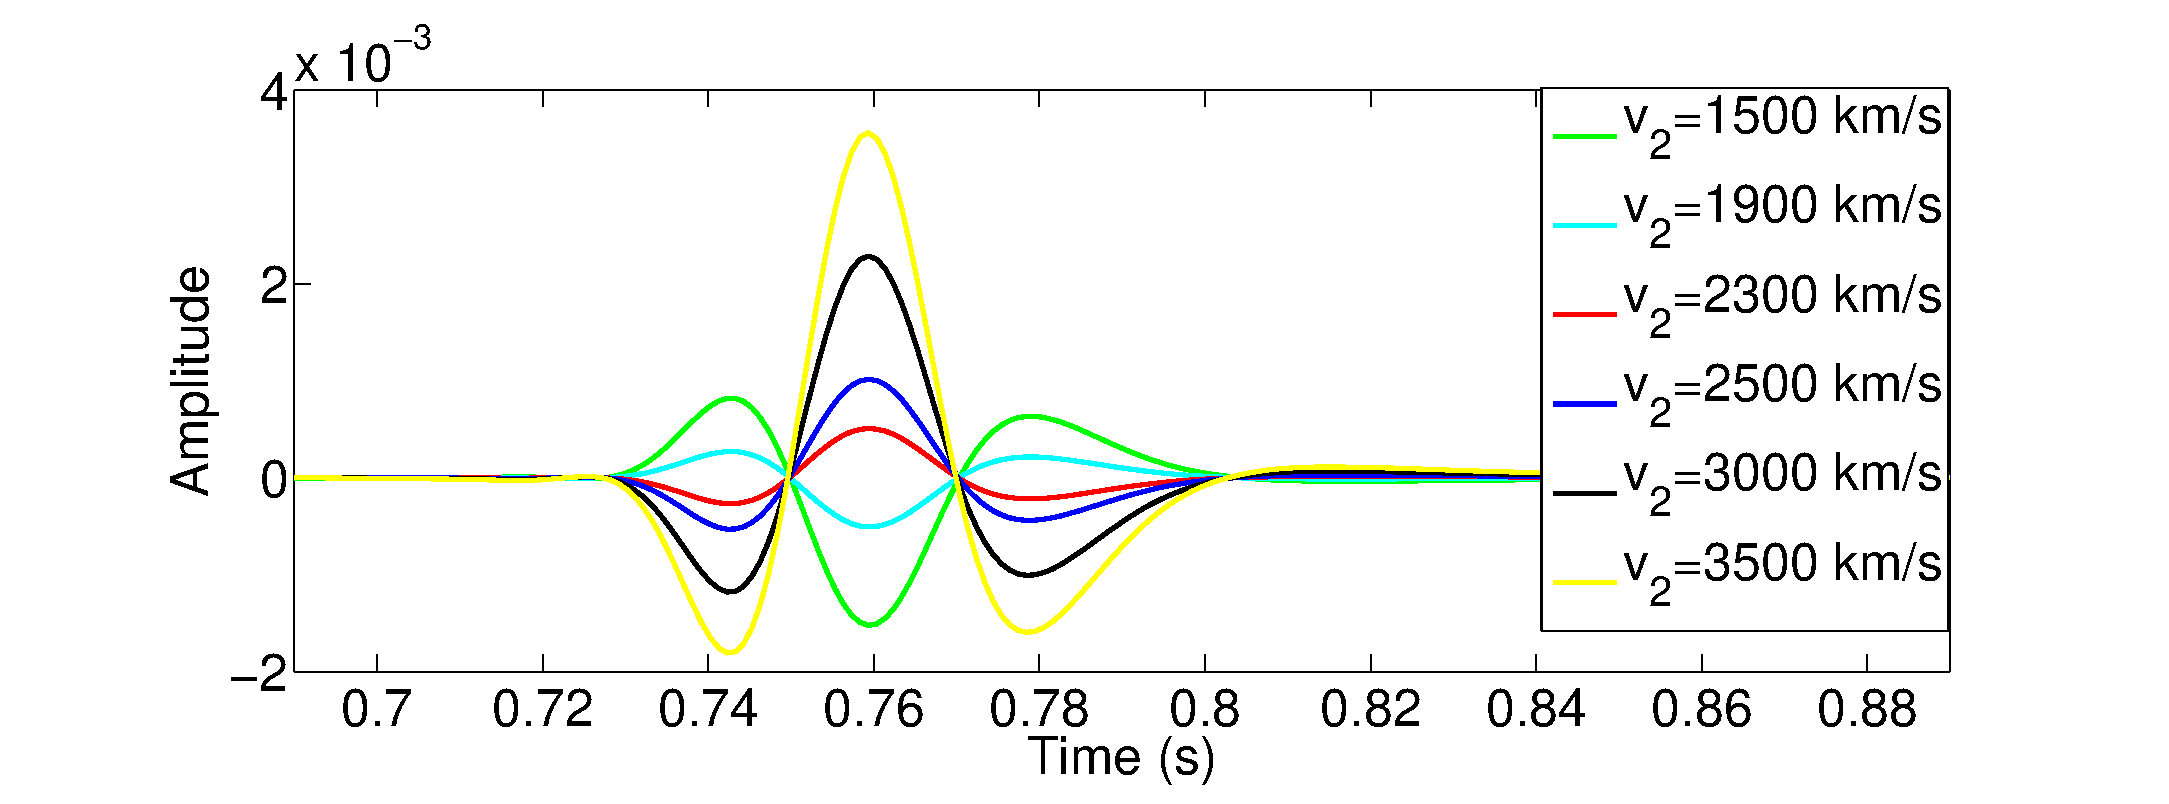
\includegraphics[width=0.92\linewidth]{figure/traces_ch41}}
    \subfigure[]{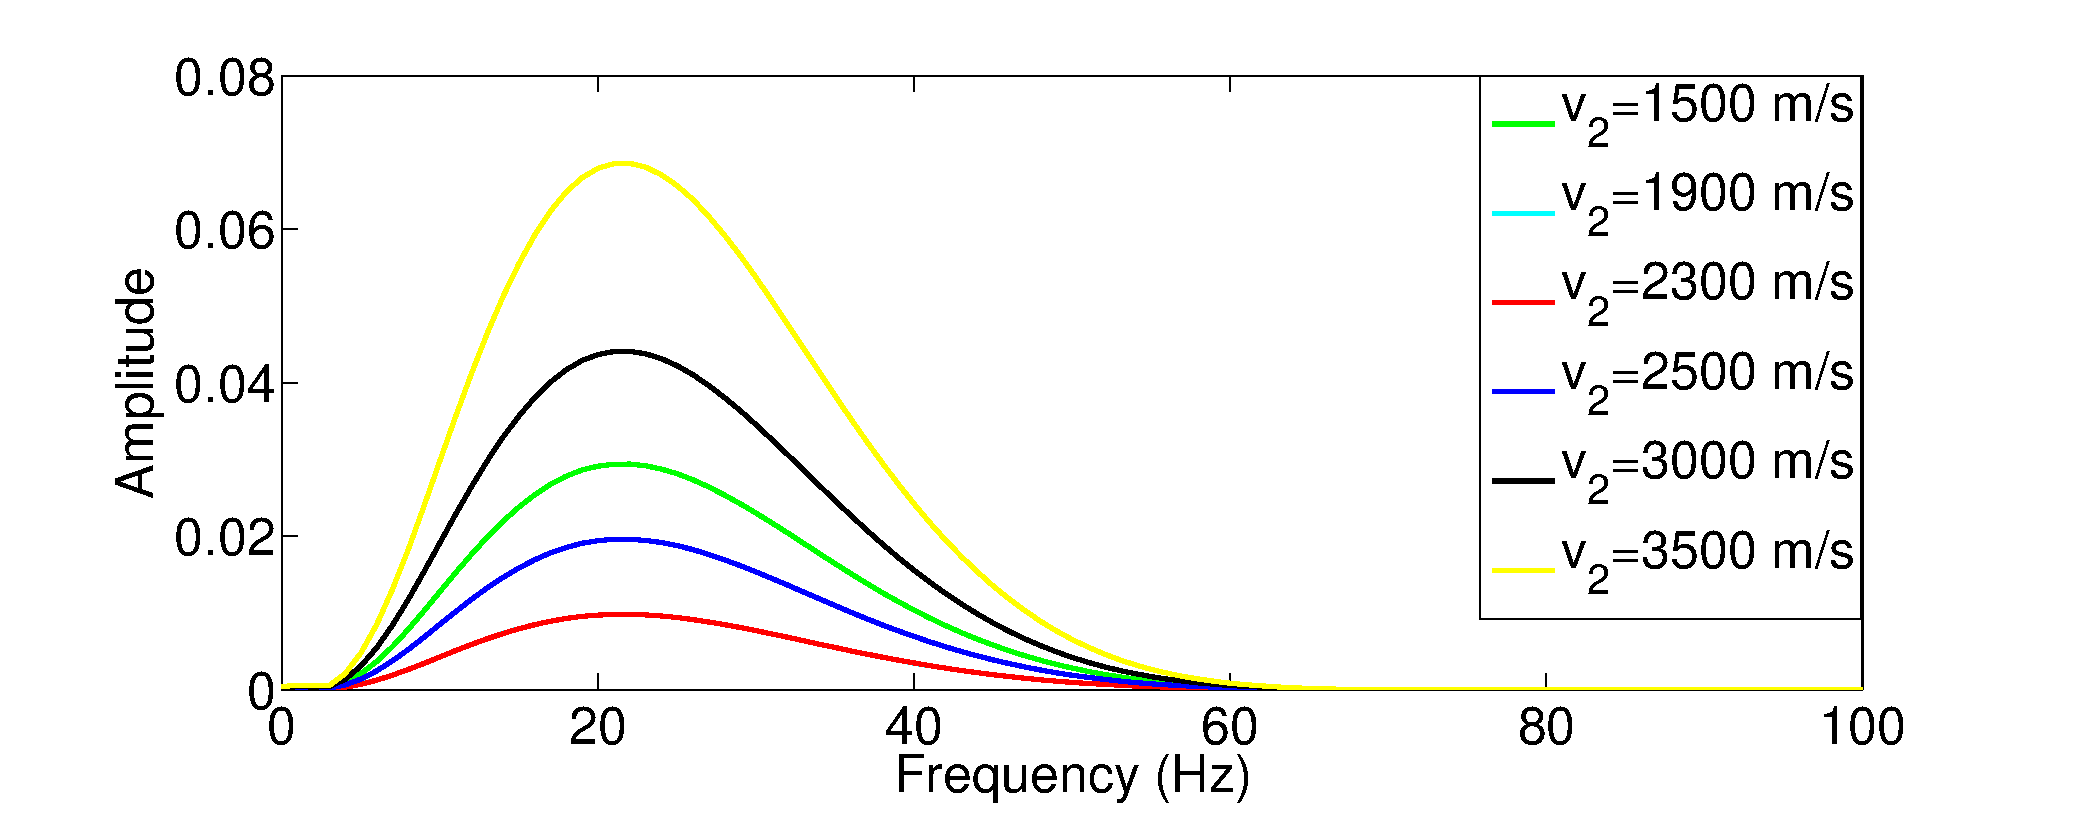
\includegraphics[width=0.92\linewidth]{figure/spectral_ch41}}
    \subfigure[]{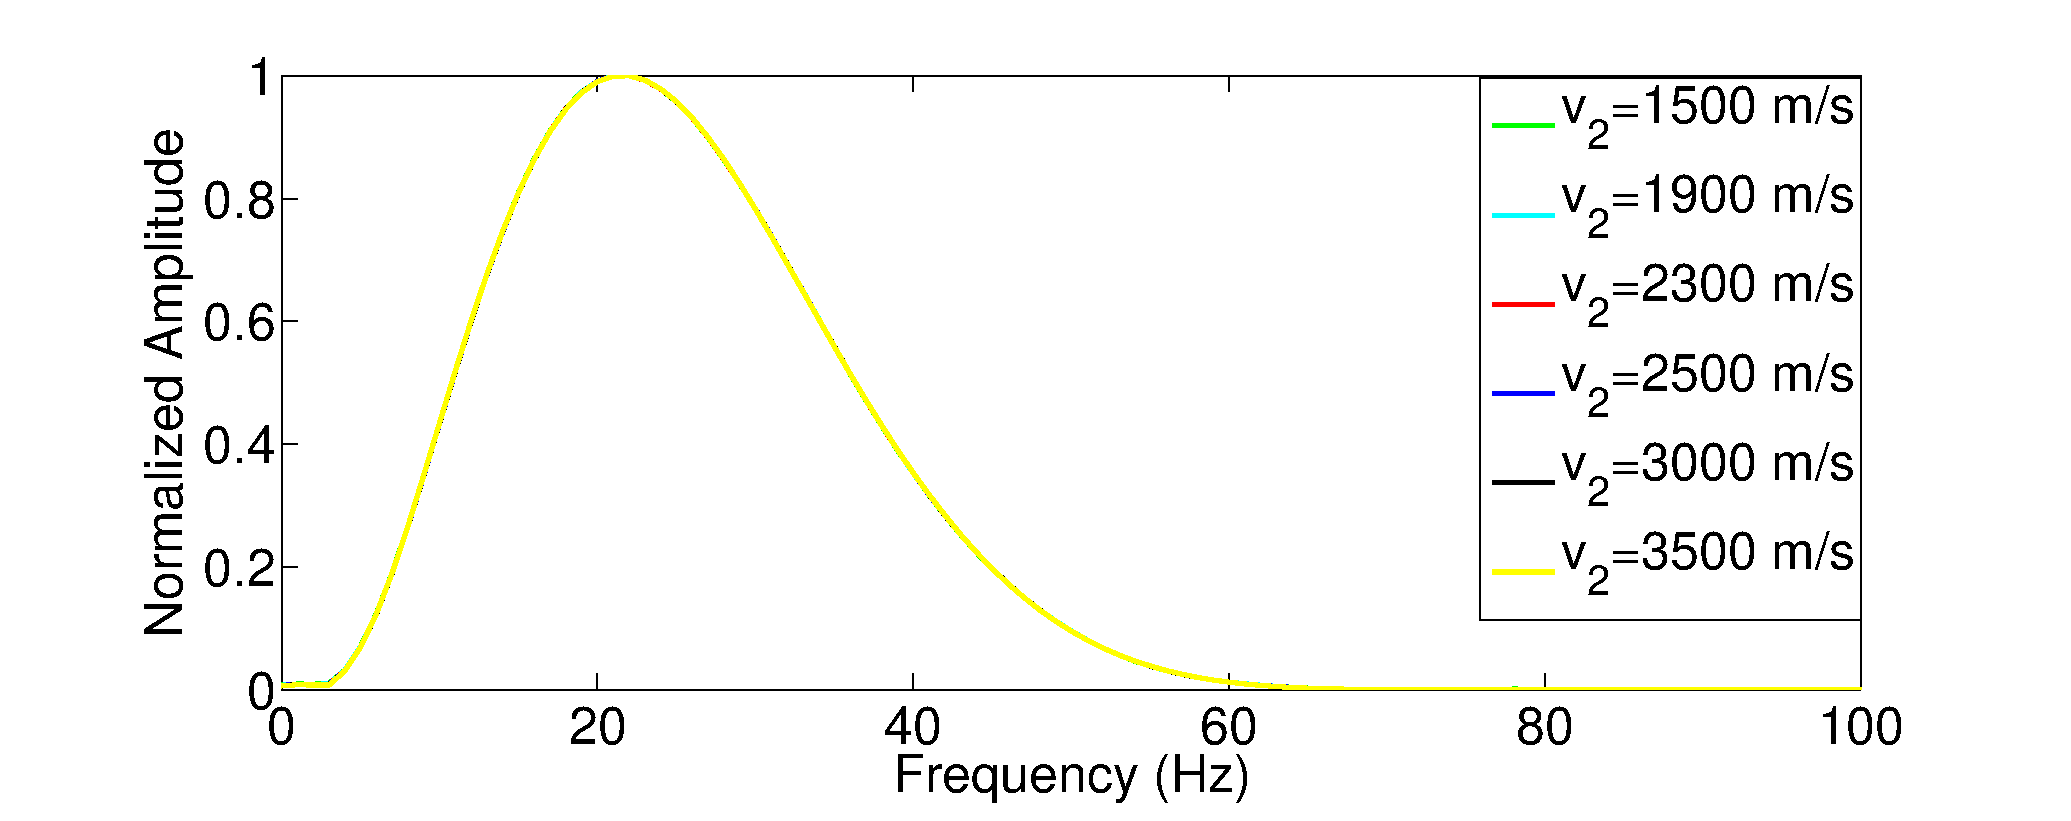
\includegraphics[width=0.92\linewidth]{figure/normalized_spectral_ch4}}
	\fcaption{两层速度结构,上层速度固定为2100m/s,下层速度从1700m/s变化到3500m/s时的Born
	正演结果,其中分离高低波数速度结构的平滑半径为8: (a)Born 正演模拟结果;
	(b)对应的振幅谱;(c)归一化振幅谱。}{Two-layer model with 2100m/s in the top layer and 
	the velocity of the bottom layer varies from 1700m/s to 3500, the smooth radius is 8 for 
	decomposition the background and perturbation velocity for the Born modeling: (a) the Born
	modeling seismic traces; (b) the corresponding amplitude spectral; (c) the normalized 
	amplitude spectral.}
    [不同速度差异的层状模型的Born模拟结果]
    \label{fig:contrast}
\end{figure*}

%%%%%%%%%%%%%%%%%%%%%%%%%%%%%%%%%%%%%

\newpage
\vspace{1.5cm}
\section{方法原理}

基于峰值频率移动目标函数的$Q$-RWI算法步骤跟波动方程走时反演(\citeA{luo.schuster:1991};
\citeA{ma.hale:2013})类似。首先需要定义一个链接函数来连接峰值频率移动残差与声压波场的
关系;其次需要定义与峰值频率移动相关的目标泛函;最后需要用粘声波方程以及链接函数来推导
目标函数对$Q$的一阶导数即梯度方向。在这一章的推导中,我们假定地震波传播满足二维时间域
SLS模型粘声波方程~\ref{eq:state}。

用$\hat{P}_f(\mathbf{x}_s,\mathbf{x}_g,t)$表示给定背景$Q$模型的模拟震相,下标$f$表示
该震相的峰值频率,峰值频率从震相的振幅谱(图~\ref{fig:q_effect}c~中黑线)中获取。
类似地,用$P_{f-f_1}(\mathbf{x}_s,\mathbf{x}_g,t)$表示同一震相峰值频率为$f-f_1$的
观测数据,其震相的振幅谱用图~\ref{fig:q_effect}c~中的蓝线表示。其中,$f_1$表示由于
$Q$不准引起的模拟数据与观测数据间峰值频率的移动,为了方便表达,这一节我们假设地震数据中
只含有单一震相,多震相的峰值频率提取方法将在下一节中给出。

给定一个足够准确的背景速度模型,模拟数据与观测数据之间相似性可以定义为:
\begin{equation}
	F_{f_1}(\mathbf{x}_s,\mathbf{x}_g,t)=\int dt P_{f-f_1}(\mathbf{x}_s,\mathbf{x}_g,t) 
	\hat{P}_f(\mathbf{x}_s,\mathbf{x}_g,t).
	\label{eq:correlation}
\end{equation}
在这一章的$Q$-RWI算法中,主要是寻求最小的峰值频率移动。对于准确的背景$Q$模型,
观测数据和模拟数据具有相同的峰值频率。换句话说,就是寻求一个移动值$f_1=\Delta f$,
使其最大化方程~\ref{eq:correlation}中的互相关函数。如果$\Delta f=0$,表明我们找到了
正确的背景$Q$模型。

因为$f_1=\Delta f$最大化了互相关函数~\ref{eq:correlation},所以$F_{f_1}(\mathbf{x}_s,
\mathbf{x}_g,t)$对$f_1$的导数在$f_1=\Delta f$处为零,即:
\begin{equation}
	\begin{aligned}
		\dot{F}_{\Delta f}(\Delta f,\tau(\mathbf{x})) &=\left[\frac{\partial F_{f_1}
	(\mathbf{x}_s,\mathbf{x}_g,t)}{\partial f_1}\right]_{f_1=\Delta f}, \\
		&= \int dt \dot{P}_{f-\Delta f}(\mathbf{x}_s,\mathbf{x}_g,t)
	\hat{P}_f(\mathbf{x}_s,\mathbf{x}_g,t)=0,
	\label{eq:connective}
	\end{aligned}
\end{equation}
式中$\dot{P}_{f-\Delta f}(\mathbf{x}_s,\mathbf{x}_g,t)=[\partial P_{f-f_1}(\mathbf{x}_s,
\mathbf{x}_g,t)/\partial f_1]_{f_1=\Delta f}$。方程~\ref{eq:connective}~即为链接函数,
链接函数作为一个中间方程来连接基础数据(声压波场)与骨架数据(频率移动残差)。因为波动方程
不能直接建立起骨架数据与模型参数的关系,所以在推导梯度时链接函数是必需的。

本章中,目标函数的定义如~\ref{eq:freq_misfit_function}~式。其梯度$\gamma(\mathbf{x})$
表示如下:
\begin{equation}
	\gamma(\mathbf{x})=\frac{\partial\mathcal{J}}{\partial \tau(\mathbf{x})}
	=-\sum_{s,g}\frac{\partial \Delta f}{\partial \tau(\mathbf{x})}
	\Delta f(\mathbf{x}_s,\mathbf{x}_g,t).
	\label{eq:gradient}
\end{equation}
从方程~\ref{eq:connective}~出发,可以得到如下三个方程:
\begin{equation}
	\begin{aligned}
		 &\dot{F}_{\Delta f}(\Delta f,\tau(\mathbf{x}))=0, \\
		&\Rightarrow \frac{\partial \dot{F}_{\Delta f}}{\partial \Delta f} 
		\frac{\partial \Delta f}{\partial \tau(\mathbf{x})} + 
		\frac{\partial \dot{F}_{\Delta f}}{\partial\tau(\mathbf{x})} =0, \\
		&\Rightarrow \frac{\partial \Delta f}{\partial \tau(\mathbf{x})} =
		-\frac{\frac{\partial \dot{F}_{\Delta f}}{\partial\tau(\mathbf{x})}}
		{\frac{\partial \dot{F}_{\Delta f}}{\partial \Delta f}},
	\end{aligned}
	\label{eq:partial_f}
\end{equation}
\begin{equation}
	\frac{\partial \dot{F}_{\Delta f}}{\partial \Delta f} = \int dt 
	\ddot{P}_{f-\Delta f}(\mathbf{x}_s,\mathbf{x}_g,t)
	\hat{P}_f(\mathbf{x}_s,\mathbf{x}_g,t)=0,
\end{equation}
\begin{equation}
	\frac{\partial \dot{F}_{\Delta f}}{\partial\tau(\mathbf{x})} = \int dt
	\dot{P}_{f-\Delta f}(\mathbf{x}_s,\mathbf{x}_g,t) 
	\frac{\partial \hat{P}_f(\mathbf{x}_s,\mathbf{x}_g,t)}{\partial \tau(\mathbf{x})}
\end{equation}
利用方程~\ref{eq:partial_f}~可以把方程~\ref{eq:gradient}~的梯度可以表示为:
\begin{equation}
	\gamma(\mathbf{x})=\sum_{s,g}\frac{\frac{\partial \dot{F}_{\Delta f}}{\partial\tau(\mathbf{x})}}
	{\frac{\partial \dot{F}_{\Delta f}}{\partial \Delta f}}\Delta f(\mathbf{x}_s,\mathbf{x}_g,t).
\end{equation}
\citeB{dutta.schuster:2016}显示地推导出了Frechet导数$[\partial \hat{P}_f(\mathbf{x}_s,
\mathbf{x}_g,t)/\partial \tau(\mathbf{x})]$,其推导过程略微麻烦。本节用伴随状态法来
推导梯度$\gamma(\mathbf{x})$,两种方法推导的结果一致。

基于峰值频率移动目标函数的$Q$-RWI满足的物理状态方法跟第三章所用的物理方程
(方程~\ref{eq:state})一致,即$\mathbf{L(m)}\mathbf{w(m)}=\mathbf{f}$。
物理状态变量$\mathbf{w}$与模型参数$\mathbf{m}$的偏导数有如下关系:
\begin{equation}
	\begin{aligned}
		&\mathbf{L(m)}\mathbf{w(m)}=\mathbf{f} \\
		&\Rightarrow \frac{\partial \mathbf{L(m)}}{\partial\mathbf{m}}\mathbf{w(m)}+
		\mathbf{L(m)}\frac{\partial\mathbf{w(m)}}{\partial\mathbf{m}}=0 \\
		&\Rightarrow \frac{\partial\mathbf{w(m)}}{\partial\mathbf{m}}=
		-\mathbf{L^{-1}(m)}\frac{\partial \mathbf{L(m)}}{\partial\mathbf{m}}\mathbf{w(m)}.
	\end{aligned}
	\label{eq:ad_state}
\end{equation}
链接函数\ref{eq:connective}可以重新写成如下表达式:
\begin{equation}
	\dot{F}_{\Delta f}=\left\langle \hat{\mathbf{w}}_f(\mathbf{x}_s,\mathbf{x}_g,t),
	\dot{\mathbf{w}}_{f-\Delta f}(\mathbf{x}_s,\mathbf{x}_g,t) \right\rangle,
\end{equation}
式中$\langle \mathbf{x},\mathbf{y}\rangle$表示向量$\mathbf{x}$,$\mathbf{y}$之间的标量积。
$\hat{\mathbf{w}}_f$和$\mathbf{w}_{f-\Delta f}$分别表示同一震相的模拟数据与观测数据。
目标函数$\mathcal{J}$的梯度满足如下推导:
\begin{equation}
	\begin{aligned}
		\frac{\partial \mathcal{J}}{\partial \tau(\mathbf{x})} &= -\sum_s \sum_g 
		\frac{\partial \Delta f}{\partial \tau(\mathbf{x})}
		\Delta f(\mathbf{x}_s,\mathbf{x}_g,t), \\
		&=\sum_s \sum_g \frac{1}{\mathbf{E}}\frac{\partial \dot{F}_{\Delta f}}
		{\partial \tau(\mathbf{x})} \Delta f(\mathbf{x}_s,\mathbf{x}_g,t), \\
		&= \sum_s \sum_g \frac{1}{\mathbf{E}}\frac{\partial}{\partial \tau(\mathbf{x})}
		\left\langle \hat{\mathbf{w}}_f(\mathbf{x}_s,\mathbf{x}_g,t), 
		\dot{\mathbf{w}}_{f-\Delta f}(\mathbf{x}_s,\mathbf{x}_g,t) \right\rangle 
		\Delta f(\mathbf{x}_s,\mathbf{x}_g,t), \\
		&= \sum_s \sum_g\left\langle \frac{\partial \hat{\mathbf{w}}_f(\mathbf{x}_s,\mathbf{x}_g,t)}
		{\partial \tau(\mathbf{x})},\dot{\mathbf{w}}_{f-\Delta f}(\mathbf{x}_s,\mathbf{x}_g,t)
		\Delta f(\mathbf{x}_s,\mathbf{x}_g,t)\frac{1}{\mathbf{E}}\right\rangle, \\
		&= -\sum_s \sum_g\left\langle \mathbf{L^{-1}}\frac{\partial \mathbf{L}}{\partial \tau(\mathbf{x})}
		\hat{\mathbf{w}}_f(\mathbf{x}_s,\mathbf{x}_g,t),\dot{\mathbf{w}}_{f-\Delta f}(
		\mathbf{x}_s,\mathbf{x}_g,t)\Delta f(\mathbf{x}_s,\mathbf{x}_g,t)\frac{1}{\mathbf{E}}\right\rangle, \\
		&=-\sum_s\left\langle\frac{\partial \mathbf{L}}{\partial \tau(\mathbf{x})}
		\hat{\mathbf{w}}_f(\mathbf{x}_s,\mathbf{x}_g,t),(\mathbf{L}^{-1})^\ast\sum_g
		\left(\dot{\mathbf{w}}_{f-\Delta f}(\mathbf{x}_s,\mathbf{x}_g,t)
		\Delta f(\mathbf{x}_s,\mathbf{x}_g,t)\frac{1}{\mathbf{E}}\right)\right\rangle, \\
		&=-\sum_s\left\langle \frac{\partial \mathbf{L}}{\partial \tau(\mathbf{x})}
		\hat{\mathbf{w}}_f(\mathbf{x}_s\mathbf{x}_g,t),
		\mathbf{w}^\ast(\mathbf{x}_s,\mathbf{x}_g,t)\right\rangle.
	\end{aligned}
	\label{eq:ad_algrithm}
\end{equation}
上式中
\begin{equation}
	\mathbf{E}=\begin{bmatrix} E_1 \cr E_2 \cr E_3 \cr E_4 \end{bmatrix}
		=\begin{bmatrix} \int dt \ddot{P}(\mathbf{x}_s,\mathbf{x}_g,t)_{obs}
		P(\mathbf{x}_s,\mathbf{x}_g,t)_{calc} \cr 
	\int dt \ddot{v}_x(\mathbf{x}_s,\mathbf{x}_g,t)_{obs}v_x(\mathbf{x}_s,\mathbf{x}_g,t)_{calc} \cr 
	\int dt \ddot{v}_z(\mathbf{x}_s,\mathbf{x}_g,t)_{obs}v_z(\mathbf{x}_s,\mathbf{x}_g,t)_{calc} \cr 
	\int dt \ddot{r}_p(\mathbf{x}_s,\mathbf{x}_g,t)_{obs}r_p(\mathbf{x}_s,\mathbf{x}_g,t)_{calc} 
		\end{bmatrix},
\end{equation}
$\mathbf{w}^\ast=\lbrack \delta\tilde{P}, \ \delta \tilde{v}_x, \ \delta \tilde{v}_z, \
\delta \tilde{r}_p, \ \tilde{P}, \ \tilde{v}_x, \ \tilde{v}_z, \ \tilde{r}_p\rbrack ^T$是物理变量
$\mathbf{w}=\lbrack P, \ v_x, \ v_z, \ r_p, \ \delta P, \ \delta v_x, \ \delta v_z, \ \delta r_p\rbrack ^T$
对应的伴随状态变量,并且满足如下伴随状态方程:
\begin{equation}
	\mathbf{L}^\ast\mathbf{w}^\ast=\mathbf{f}^\ast,
\end{equation}
式中$\mathbf{L}^\ast$是粘声波方程正传算子$\mathbf{L}$的伴随算子且满足~\ref{eq:ad_operator}~式;
$\mathbf{f}^\ast$为伴随源,满足如下关系式:
\begin{equation}
	\mathbf{f}^\ast=\begin{bmatrix} 0 \cr 0\cr 0\cr 0\cr
		-\sum_g\left(\dot{P}(\mathbf{x}_s,\mathbf{x}_g,t)_{obs}
		\Delta f(\mathbf{x}_s,\mathbf{x}_g,t)\frac{1}{E_1}\right) \cr
		-\sum_g\left(\dot{v}_x(\mathbf{x}_s,\mathbf{x}_g,t)_{obs}
		\Delta f(\mathbf{x}_s,\mathbf{x}_g,t)\frac{1}{E_2}\right) \cr
		-\sum_g\left(\dot{v}_z(\mathbf{x}_s,\mathbf{x}_g,t)_{obs}
		\Delta f(\mathbf{x}_s,\mathbf{x}_g,t)\frac{1}{E_3}\right) \cr
		-\sum_g\left(\dot{r}_p(\mathbf{x}_s,\mathbf{x}_g,t)_{obs}
		\Delta f(\mathbf{x}_s,\mathbf{x}_g,t)\frac{1}{E_4}\right) 
	\end{bmatrix}.
\end{equation}
在实际勘探中,假设我们只接收到压力波场,伴随源简化为\\
 $\mathbf{f}^\ast=\lbrack 0, \ 0, \ 0, \ 0, \
\Delta P(\mathbf{x}_s,\mathbf{x}_g,t), \ 0, \ 0, \ 0\rbrack ^T$,其中
$\Delta P(\mathbf{x}_s,\mathbf{x}_g,t)=(1/E_1)\dot{P}(\mathbf{x}_s,\mathbf{x}_g,t)_{obs}
 \\ \Delta f(\mathbf{x}_s,\mathbf{x}_g,t)$表示为残差道,对应于常规波形反演的数据残差伴随源。
由方程~\ref{eq:ad_algrithm}~可以得到目标函数对模型参数的梯度:
   \begin{equation}
    \begin{aligned}
        \frac{\partial \mathcal{J}}{\partial \tau} &= -\langle\frac{\partial \mathbf{L}}{\partial\tau}
        \mathbf{w},\mathbf{w}^\ast \rangle \\
        &= {K_0(\frac{\partial v_x}{\partial
        x}+\frac{\partial v_z}{\partial
    z})(-\delta\tilde{P}+\frac{1}{\tau_\sigma}\delta\tilde{r}_p)} \\
    &{+K_0(\frac{\partial \delta v_x}{\partial x}+\frac{\partial \delta
        v_z}{\partial z})(-\tilde{P}+\frac{1}{\tau_\sigma}\tilde{r}_p)} \\
        &{+\delta K(\frac{\partial v_x}{\partial x}+\frac{\partial v_z}{\partial
        z})(-\tilde{P}+\frac{1}{\tau_\sigma}\tilde{r}_p)}.
    \end{aligned}
    \label{eq:gradient1}
    \end{equation}

基于振幅匹配的$Q$-RWI梯度(\ref{eq:gradient}式)与基于峰值频率移动目标函数的$Q$-RWI的梯度
有相同的表达式。而且伴随方程的形式也相同,只是伴随源不同,前者为波形数据的残差,后者为峰值
频率残差与观测数据对频率导数的加权。由于没有显示的表达式来求取观测数据对频率的导数
$\dot{P}_{f-\Delta f}(\mathbf{x}_s,\mathbf{x}_g,t)$和$\ddot{P}_{f-\Delta f}(\mathbf{x}_s,
\mathbf{x}_g,t)$,在伴随方程的实际求解过程中,\citeB{dutta.schuster:2016}用峰值频率移动残差
加权观测数据作为伴随源,从而忽略了$\dot{P}_{f-\Delta f}$以及除数因子$E_1$。
理论数据和实际数据实验都证实了上述近似的合理性(\citeA{dutta.schuster:2016}),本文也将
采样上述近似来处理伴随源。

计算出梯度之后,用第三章的迭代流程即可更新背景$Q$模型。


\vspace{0.5cm}
\section{多震相反射数据峰值频率提取}
\vspace{0.5cm}
在实际地震勘探中,接收到的反射数据往往具有多个反射震相,而用常规Fourier变换计算出的振幅谱
是所有地震相特征的总体体现。用反射数据进行反演时,反射震相的匹配一直是一个研究点。在反射
波层析中,\citeB{wang.rao:2009}用层剥离的方法来求取各反射层的走时。在波动方程反射走时反演
中,\citeB{zhang.schuster:2011}用局部相关法,而\citeB{ma.hale:2013}
用波形动态解缠(dynamic warping)法来提取反射波各震相的走时差。
多震相反射数据峰值频率的提取首先需要知道沿时间方向的局部频率信息即时频谱。

时频谱的求取方法有很多大致可分为两类,一类基于瞬时频率求取,另一类是通过各频率分量分解
来获取时频谱。基于瞬时频率的方法是将一维时间序列的地震道变为一维频率序列数据,而频率分量分解
法是把一维时间序列地震道变换到二维的时间-频率域中。\citeB{taner:1979}首次用Hilbert变换
来求取瞬时频率,\citeB{poggiagliolmi.vesnaver:2014}同样基于Hilbert变换提出了不依赖
人为定义参数的瞬时频率求取方法。另外,\citeB{fomel:2007}在正则化反演的框架下定义了
局部频率。

地震道频率分量分解法在时频分析中被广泛应用,其中最简单、被广泛应用的方法就是短时Fourier
变换(STFT)。然而STFT产生的时频谱在整个时间频率空间的分辨率是固定的(\citeA{cohen:1995})。
为了获得可变的分辨率,\citeB{pinnegar.mansinha:2003}用任意的可变形状的窗函数进行S变换来处理地震数据。
除了Fourier基函数,连续小波变换(CWT)用小波基函数来分析地震数据的时频信息
(\citeA{chakraborty.okaya:1995};\citeA{sinha:2005};\citeA{kazemeini:2009})。
为了通过匹配地震小波的时频信息来灵活地表示信号的结构,学者们提出了匹配追踪法并将其
应用到了含气储层的检测(\citeA{wang:2007})和古河道检测(\citeA{liu.marfurt:2007})中。
在匹配追踪法中,用户需要自定义许多地震小波参数如振幅、时间延迟、尺度、频率等,过多的
参数选择使得匹配追踪法的迭代非常缓慢。\citeB{liu.fomel:2013}在正则化最小二乘反演的框架下
提出了一种用Fourier基函数来匹配目标信号的频率分量分解方法。其分解方法是可逆的,且
比传统的S变换更灵活,在地震数据面波去燥方面有很好的运用效果。

本文提取的是各震相的峰值频率,对时间-频率的分辨率要求不是很高。用简单的滑动时窗Fourier
变换即短时Fourier变换(\citeA{allen:1977})即可满足要求。时窗的选取需要四个参数:
时窗长度、每一段重叠样本数、做Fourier变换的长度以及窗函数。时窗长度、样本重叠数和窗函数
是对完整地震道震相截取参数,Fourier变换长度决定了频谱的分辨率。

\begin{figure*}[!htbp]
    \centering
    \subfigure[]{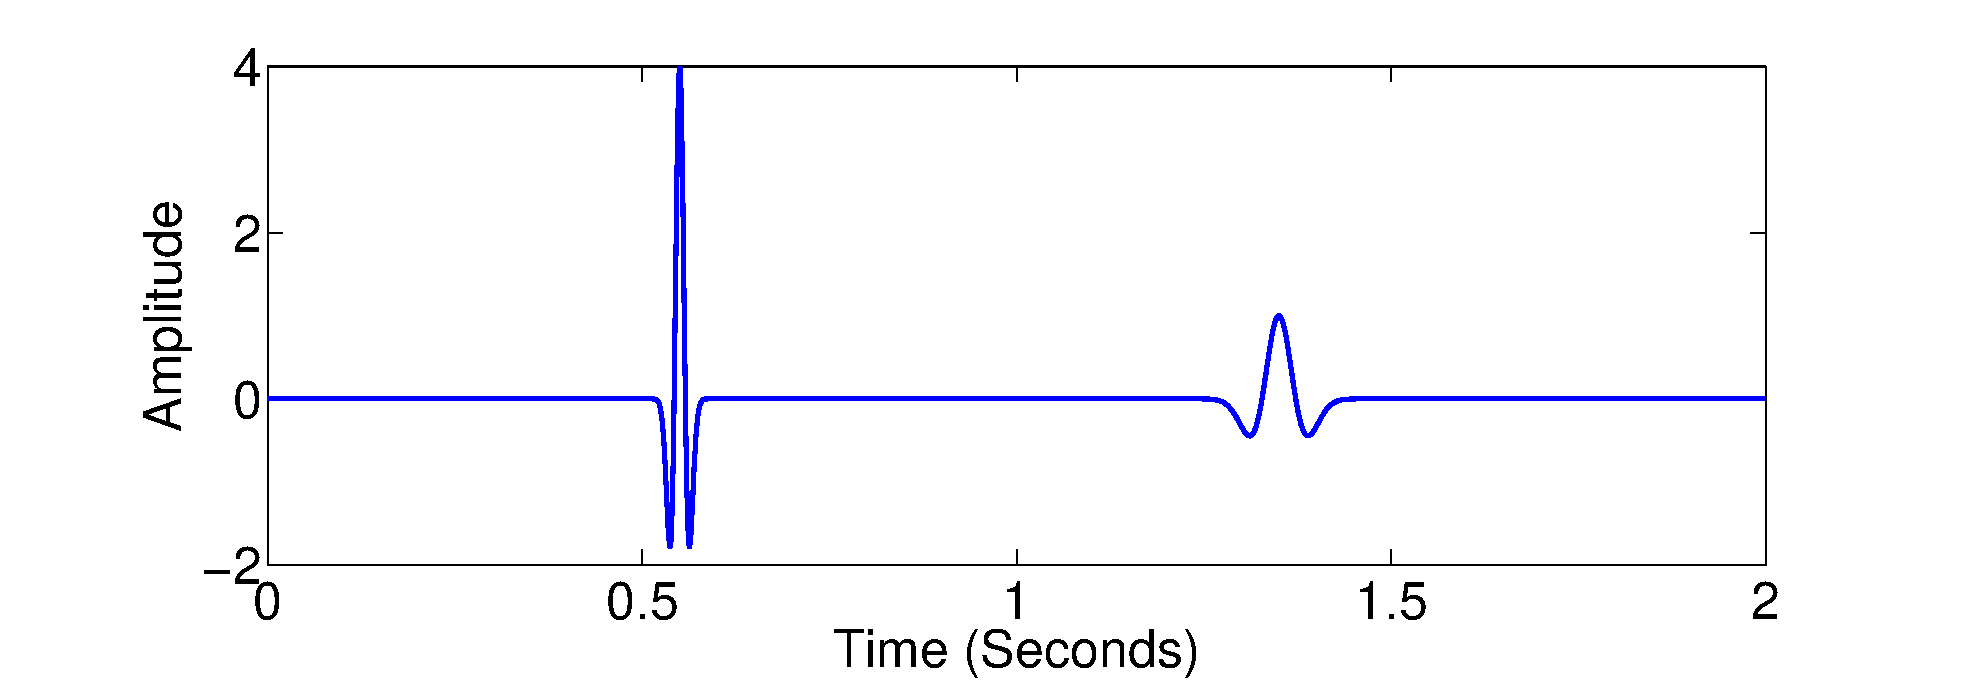
\includegraphics[width=0.9\linewidth]{figure/ricker}}
    \subfigure[]{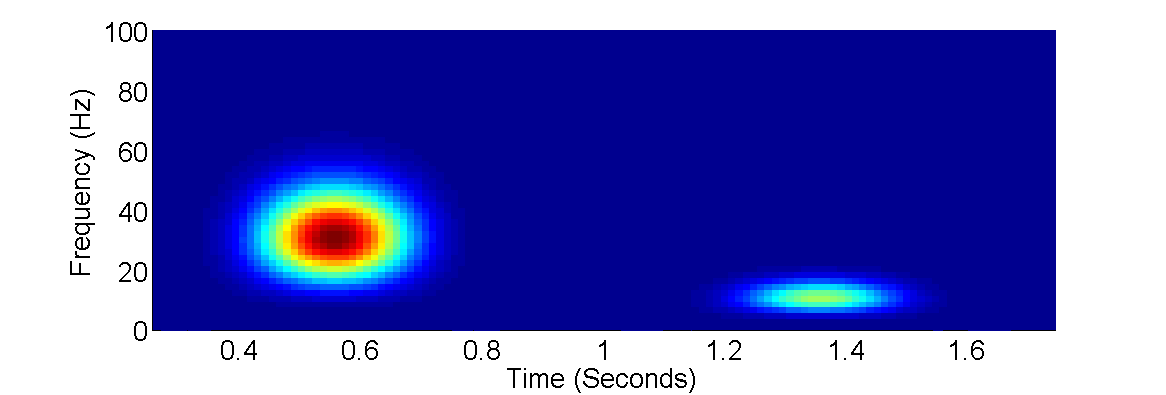
\includegraphics[width=0.9\linewidth]{figure/ricker_stft}}
    \fcaption{短时Fourier变换:(a)分别在0.55s、1.35s处用振幅为4主频
	为30Hz以及振幅为1主频为10Hz的Ricker子波合成地震道数据;(b)合成地震道对于的
	短时Fourier谱。}{The effects of STFT: (a) Sythetic seismic trace with Ricker 
	wavelet of 30Hz peak frequency at 0.55s and 10Hz peak frequency at 1.35s, the
	amplitudes of wavelet are 4 and 1, respectively; (b) the STFT spetrum.}
    [短时Fourier变换]
    \label{fig:stft_effect}
\end{figure*}
图~\ref{fig:stft_effect}a 是分别用振幅为4主频为30Hz以及振幅为1主频为10Hz的Ricker子
波在0.55s和1.35s处合成的地震记录。图~\ref{fig:stft_effect}b 展示了其对应的STFT谱,
从图中可以看出STFT很好的刻画了地震道的时频信息,而且从谱中可以很容易的拾取出两地震
相的峰值频率。

图~\ref{fig:peak_frequency}是用第三章所用的层状模型
(图~\ref{fig:lens_model})所做的单炮实验。其中图~\ref{fig:peak_frequency}a是用
真实$Q$模型计算出的观测炮记录,图~\ref{fig:peak_frequency}b是用背景$Q$模型计算
的模拟炮记录。由于深部强衰减的影响,观测炮记录第四个同相轴的能量明显弱于对应
的模拟数据,同时观测数据的峰值频率(图~\ref{fig:peak_frequency}c)相较于
模拟数据的峰值频率(图~\ref{fig:peak_frequency}d)有明显的下移。
图~\ref{fig:peak_frequency}e展示了模拟数据与观测数据的峰值频率残差,
图~\ref{fig:peak_frequency}f展示了其基于峰值频率移动目标函数的伴随源。
在该实验中,速度的低波数成分是准确的,而高波数成分是由拾取成像剖面获取的。
因此只保证了高波数速度位置的准确性,而其扰动量的大小以及分布形状是不准确的。
从伴随源的形状和能量分布以及残差道信息可以看出用STFT提取峰值频率是可行的,
且峰值频率目标函数确实可以降低$Q$-RWI对速度高波数成分的依赖性。

\begin{figure*}[!htbp]
    \centering
    \subfigure[]{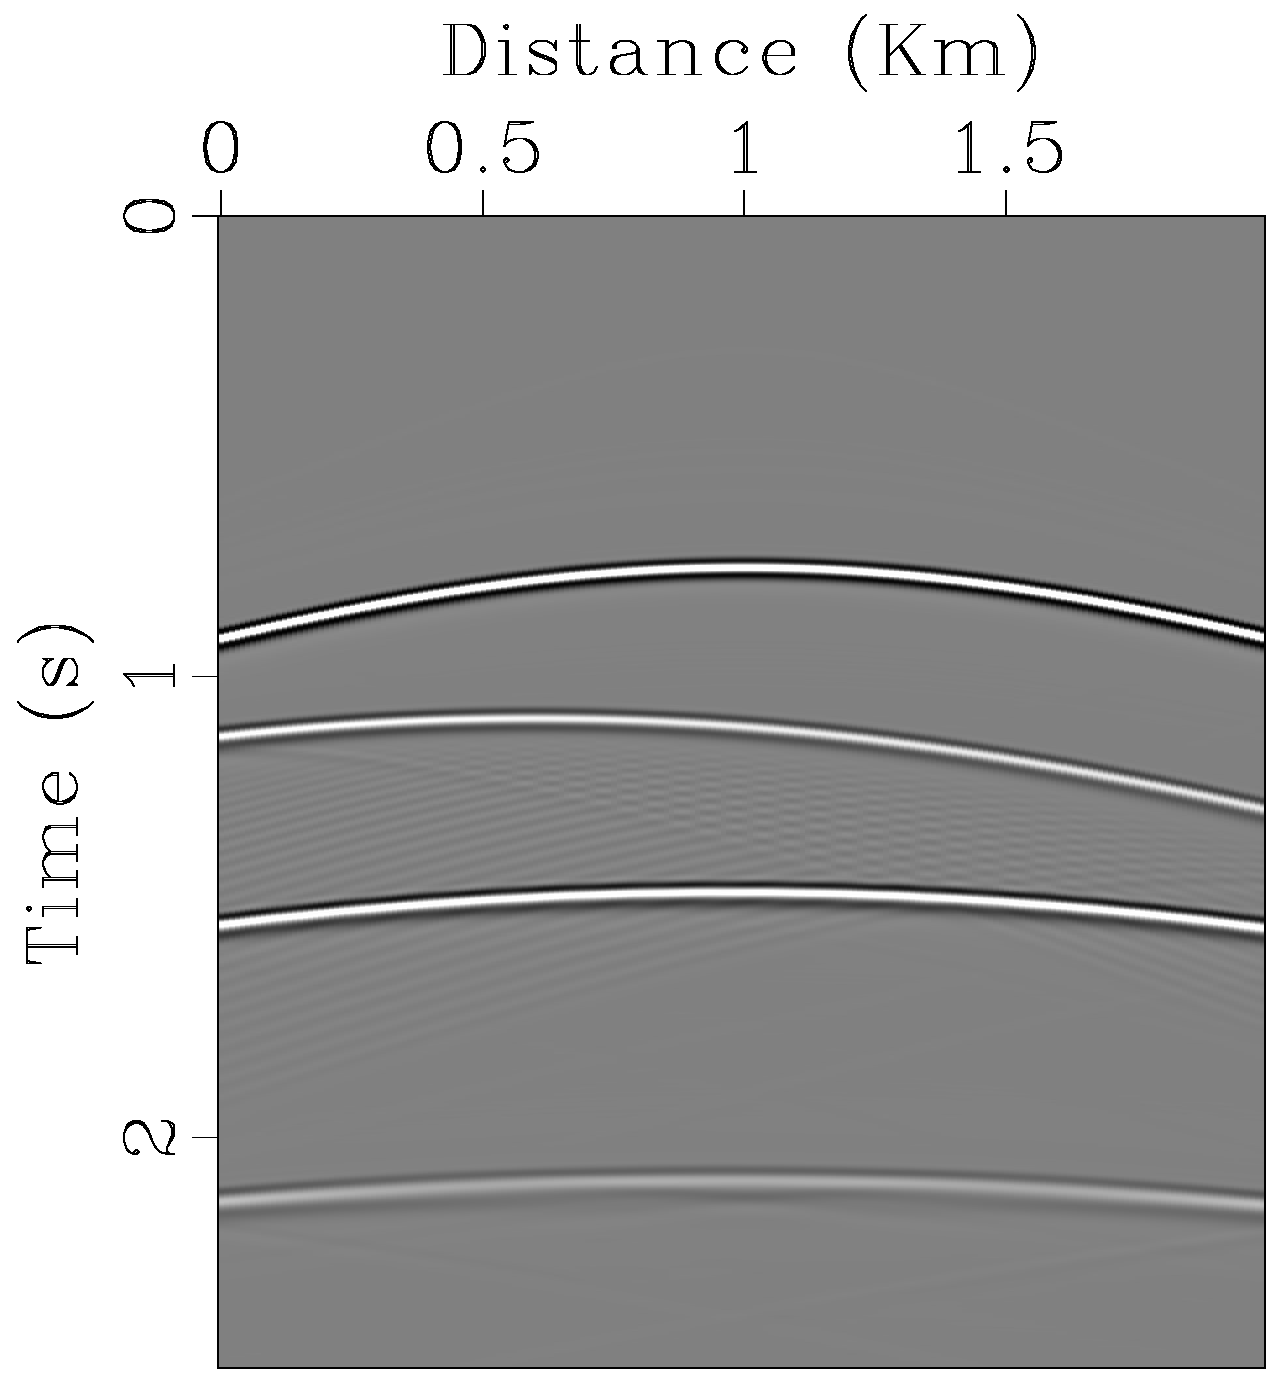
\includegraphics[width=0.40\linewidth]{figure/record_shot15}}
    \subfigure[]{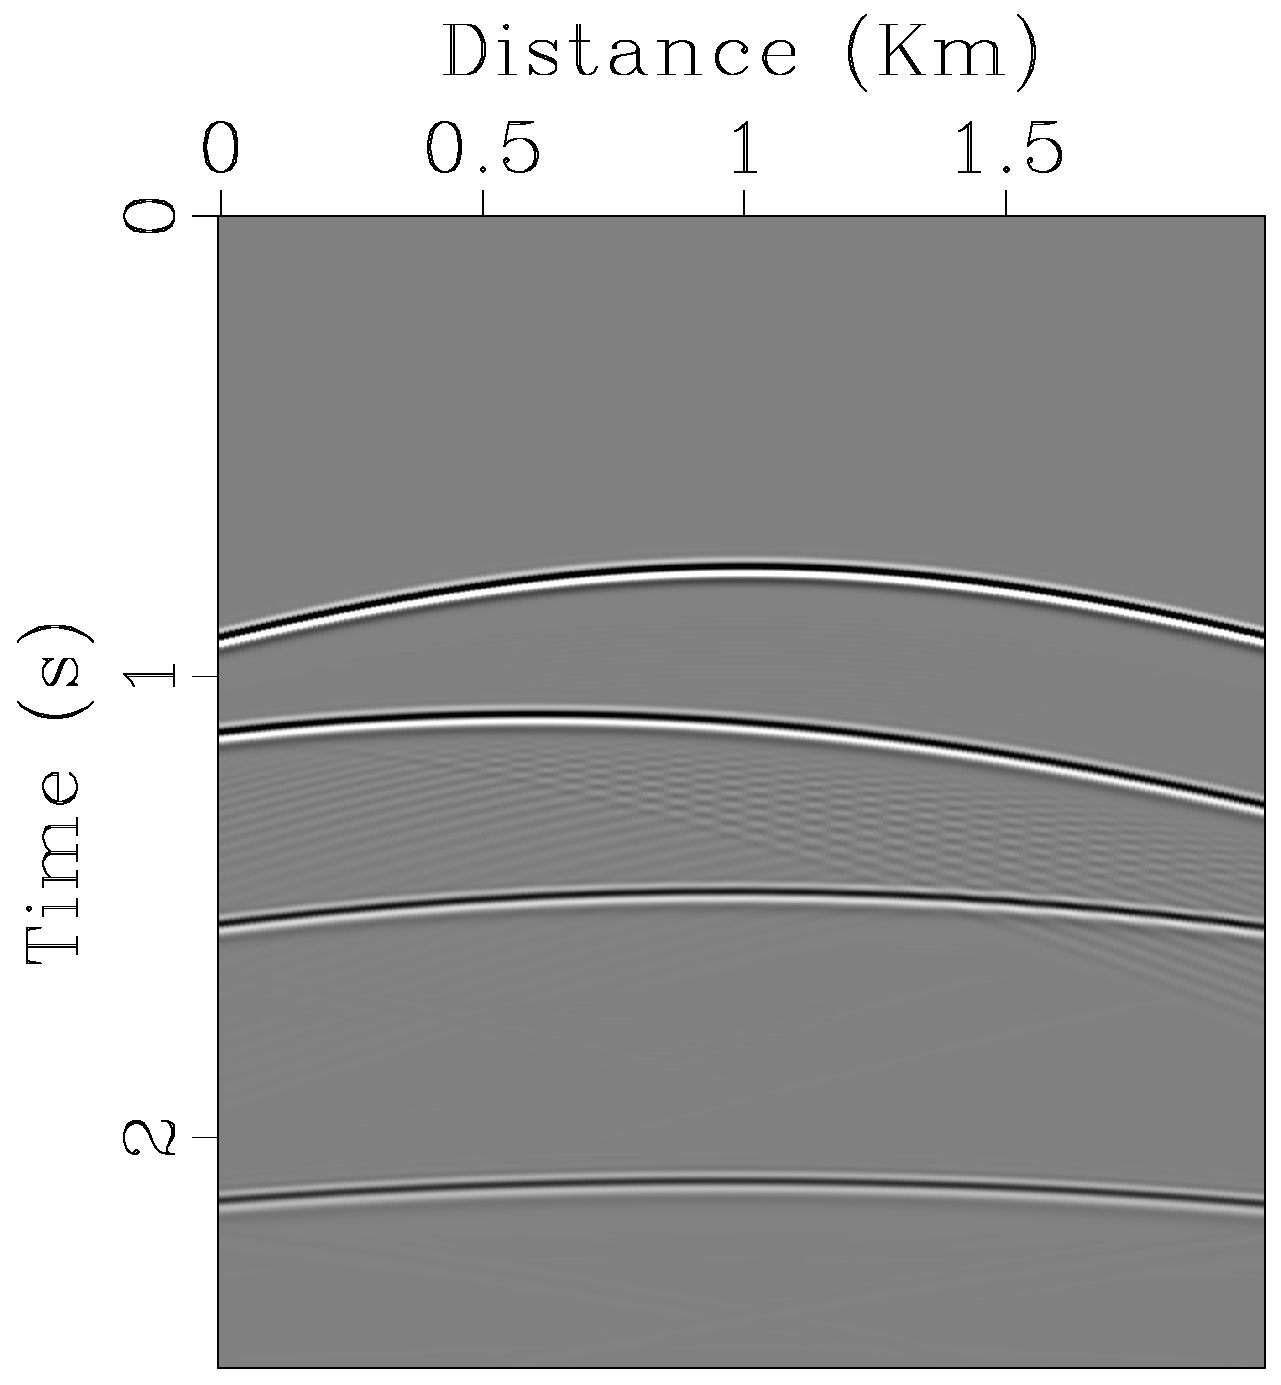
\includegraphics[width=0.40\linewidth]{figure/record_shot15_iter0}}
    \subfigure[]{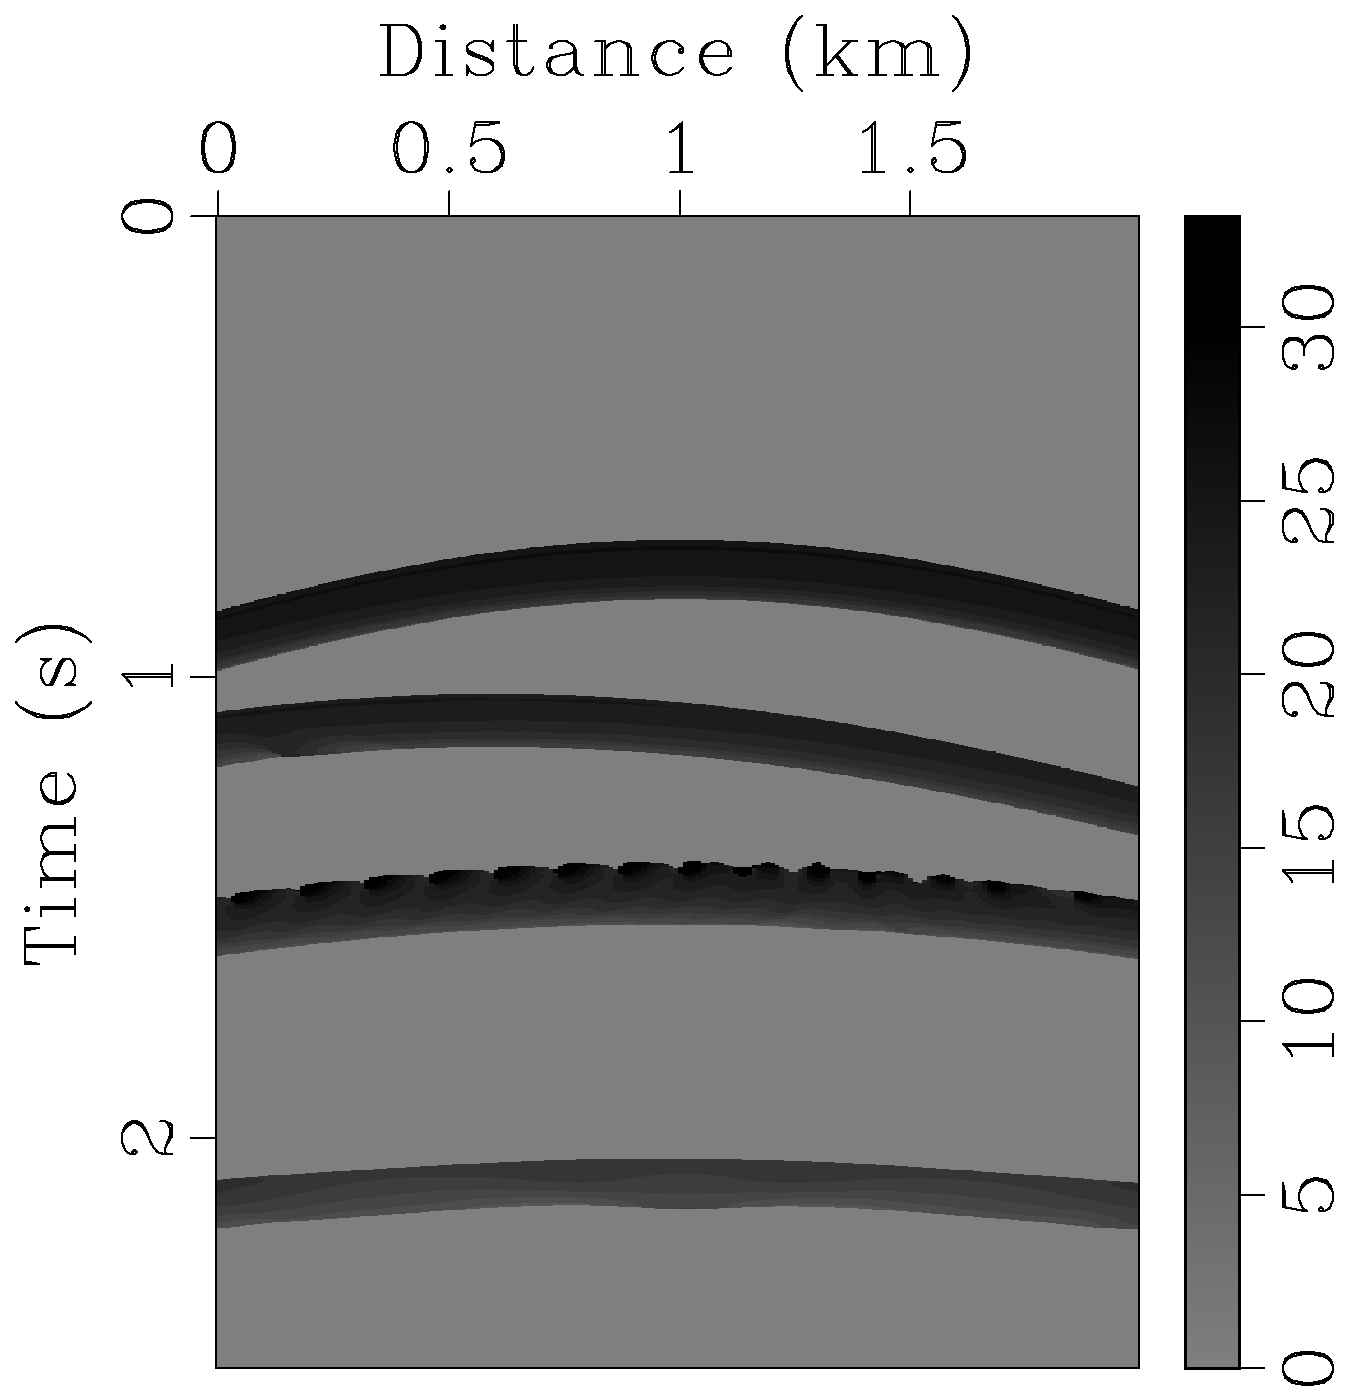
\includegraphics[width=0.40\linewidth]{figure/fpeak_obs}}
    \subfigure[]{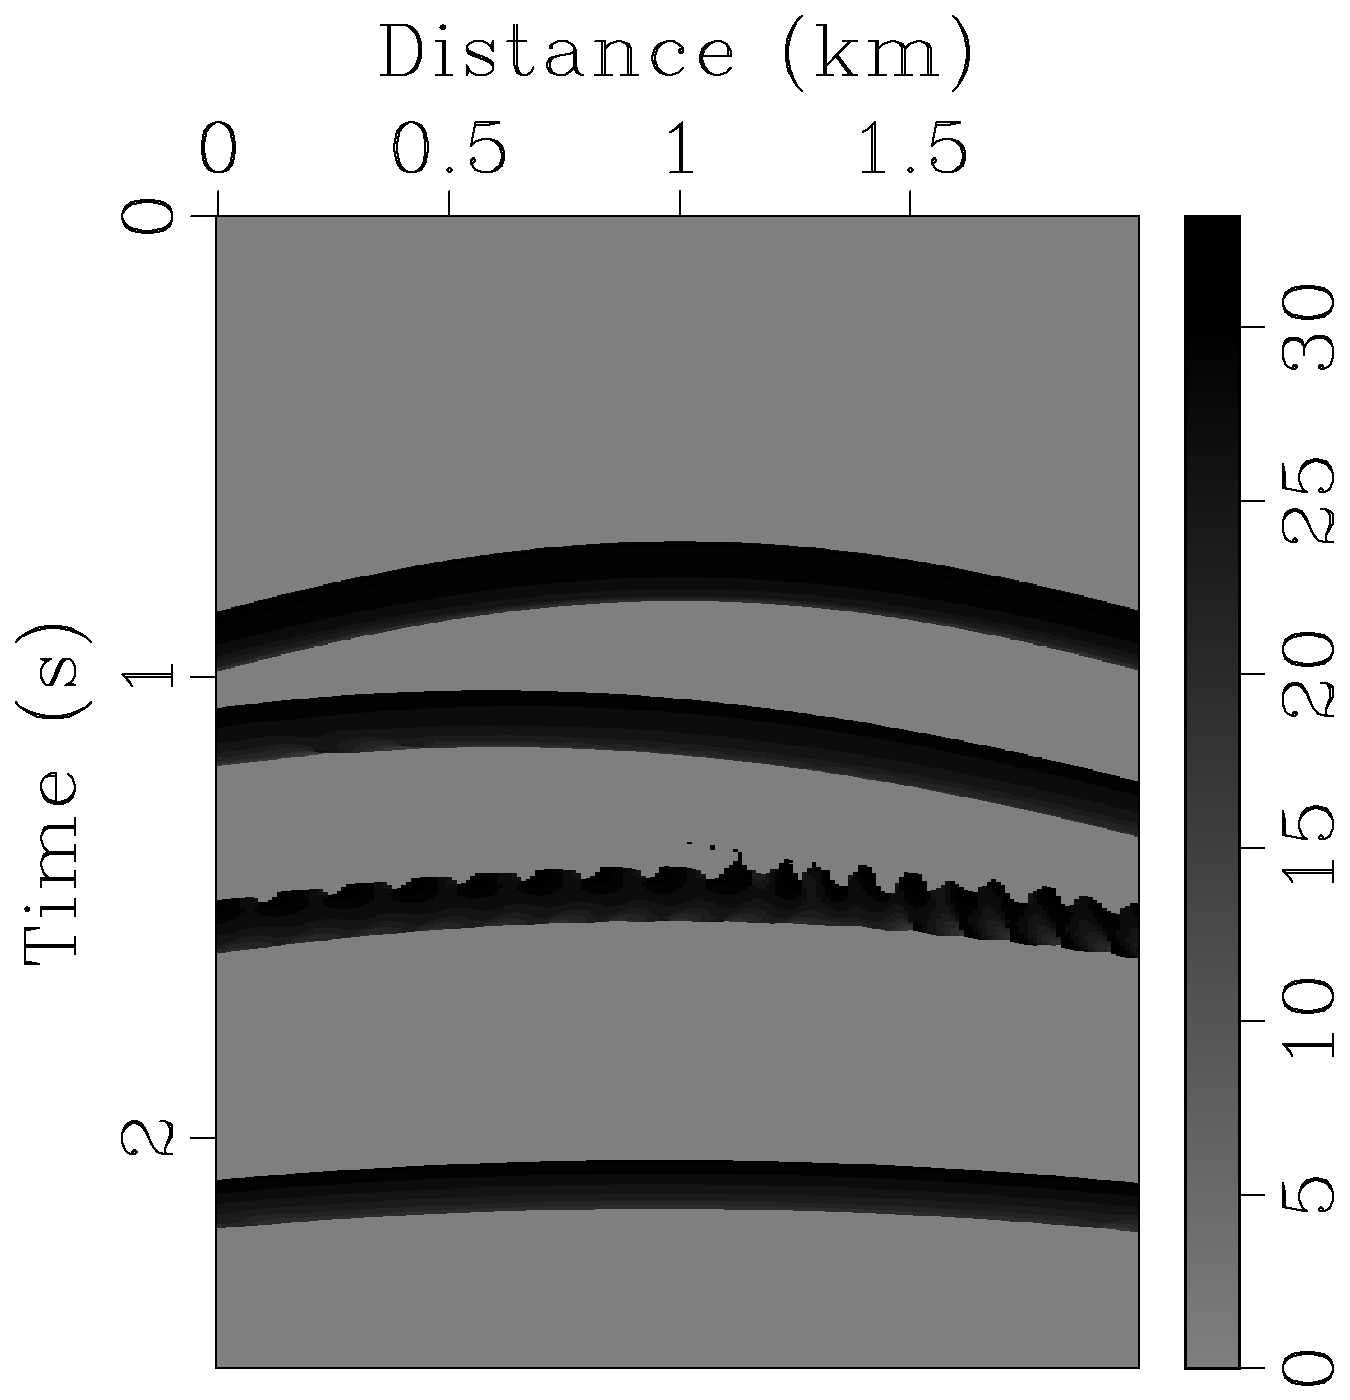
\includegraphics[width=0.40\linewidth]{figure/fpeak_cal}}
    \subfigure[]{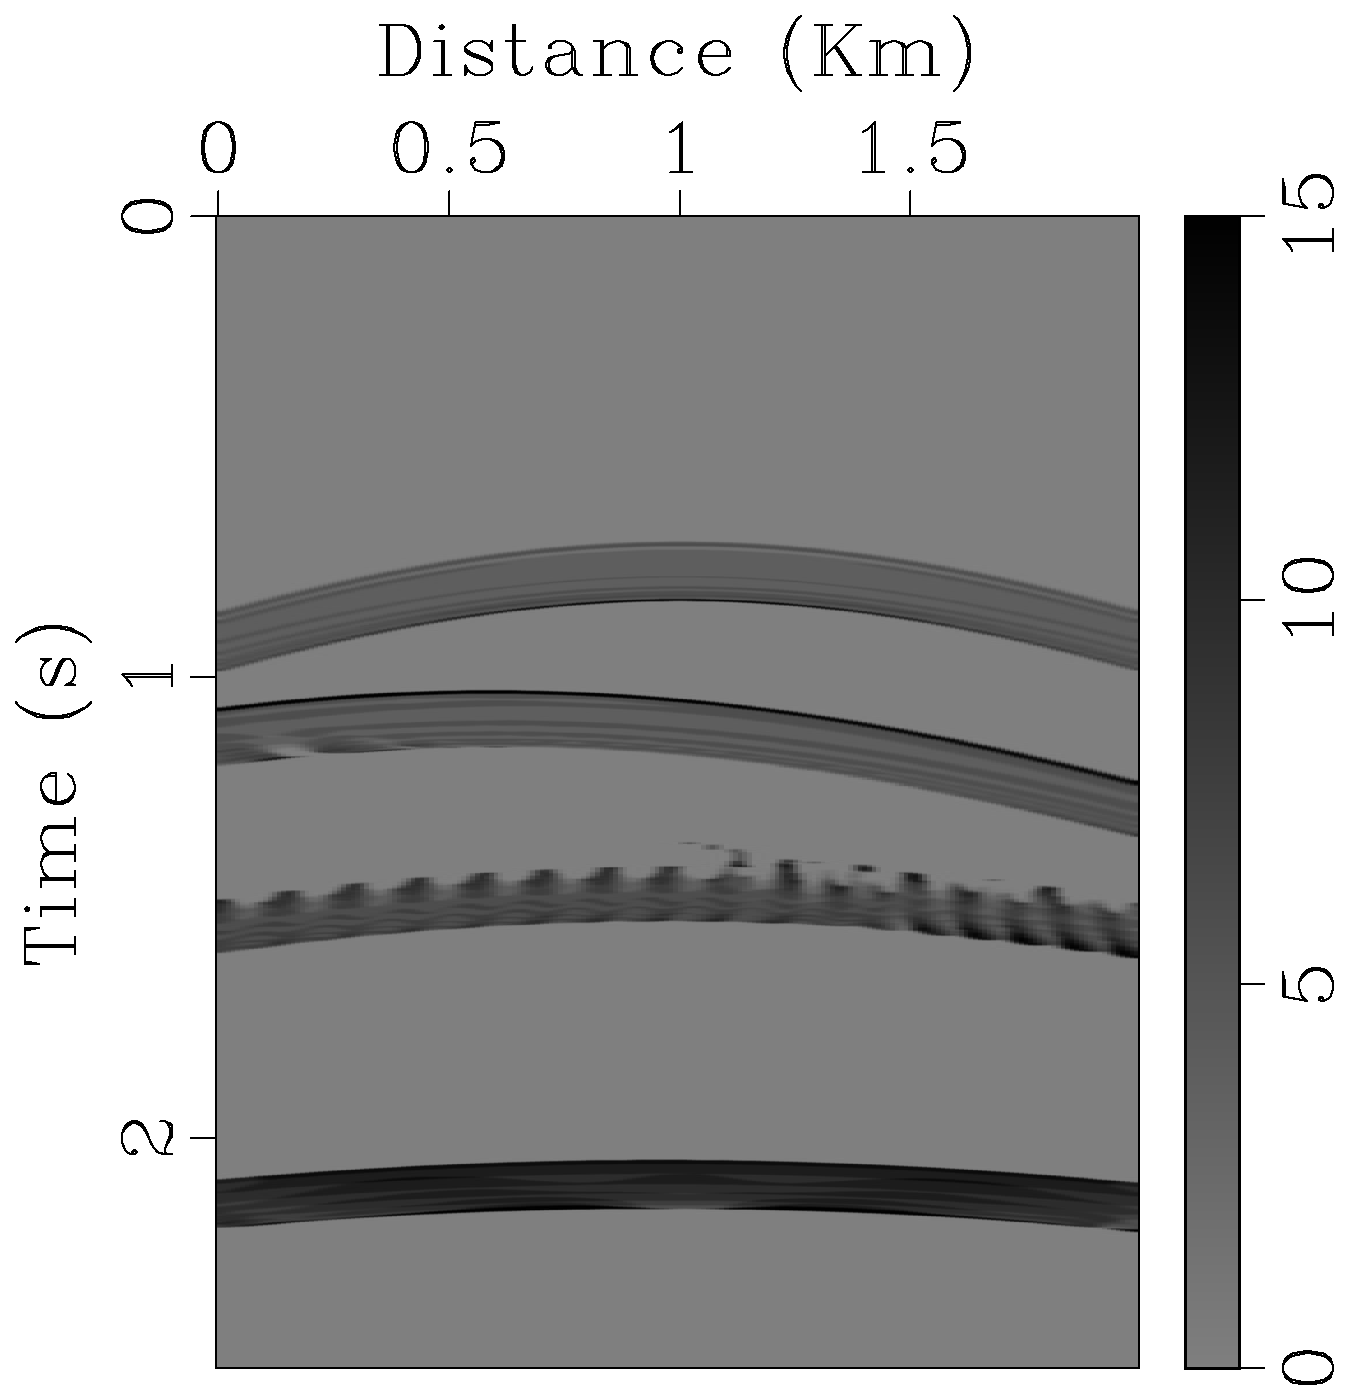
\includegraphics[width=0.40\linewidth]{figure/df2}}
    \subfigure[]{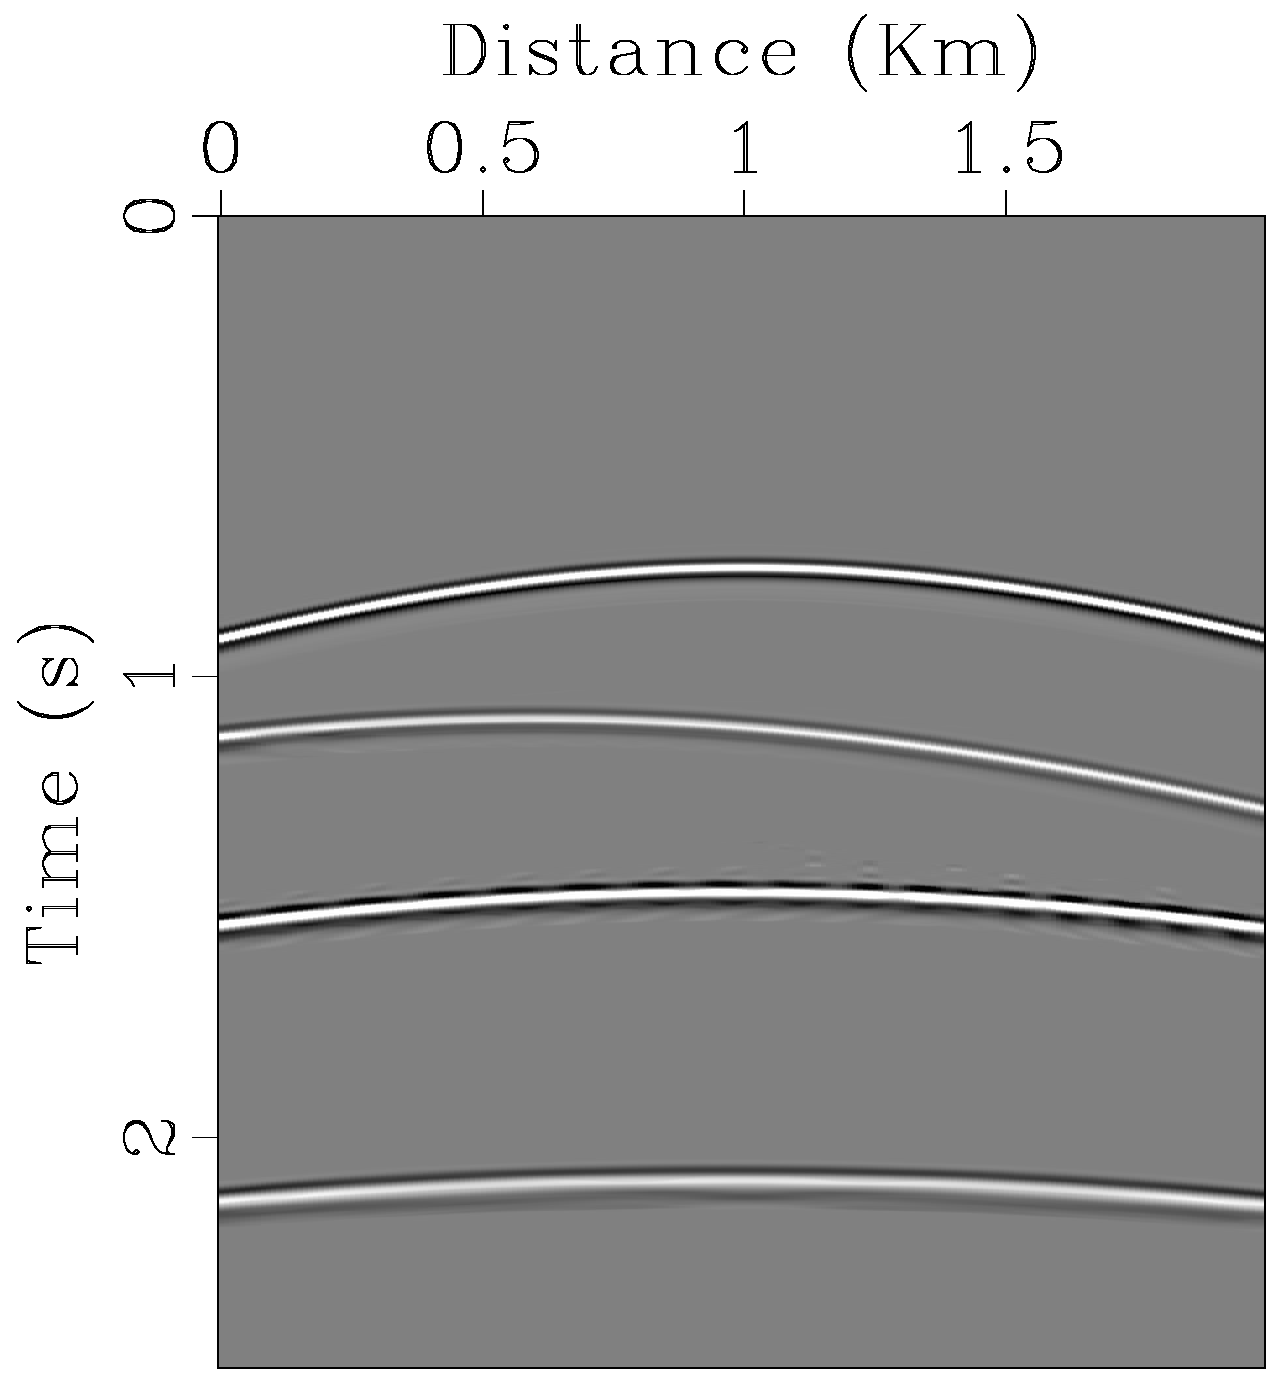
\includegraphics[width=0.40\linewidth]{figure/adsource}}
	\fcaption{短时Fourier变换提取地震数据的峰值频率:(a)观测数据;(b)模拟数据;(c)观测
	数据的峰值频率;(d)模拟数据的峰值频率;(e)峰值频率残差;(f)伴随源。}
	{Extracting the peak frequency of seismic data using STFT: (a) observed seismic data; 
	(b) calculated seismic data; (c) peak frequency of observed data; (d) peak frequency of 
	calculated data; (e) the residual frequency trace; (f) the corresponding adjoint source.}
    [短时Fourier变换提取地震数据的峰值频率]
    \label{fig:peak_frequency}
\end{figure*}

\newpage
\vspace{0.5cm}
\section{数值实验}

为了便于对比,本节继续采用第三章所用的层状模型(图~\ref{fig:lens_model}a)来验证基于峰值频率
移动目标函数的$Q$-RWI的正确性。模型大小的设置、观测系统的布置、震源子波以及初始模型的选取均
与第三章数值实验相同。本节所用的观测数据由Born正演产生,Born正演的背景模型由真实速度模型
平滑16个网格产生,其扰动模型是真实速度模型与背景模型的差。在进行反演时假设背景速度
模型已知,扰动模型选用真实速度模型与其平滑4个网格的平滑模型的差。

图~\ref{fig:lens_fmodel}c展示了基于峰值频率移动目标函数的$Q$-RWI反演结果,其反演结果与基于
振幅残差目标函数的$Q$-RWI结果(图~\ref{fig:lens_fmodel}b)基本相同。经过15次迭代之后,中深部的
$Q$异常基本得到恢复。图~\ref{fig:fchouxian}分别对比了$x=1$km、2km、3km处的伪井曲线。伪井对比
结果进一步证明了峰值频率移动目标函数在$Q$-RWI反演中的可行性。同时从抽线结果中可以看出只修改
目标函数并不能改变RWI在浅层因缺少覆盖数据而导致的多解性。多数据融合如反射数据和透射数据相
结合即可解决这种反问题的多解性。在强衰减处$x=2$km处(图~\ref{fig:fchouxian}b),基于振幅残差
目标函数的反演结果比基于峰值频率移动目标函数的反演结果分辨率高,这是因为振幅残差考虑了全波信息
而峰值频率只是地震数据的一个属性,同时这一结果也与目标函数的性态
(图~\ref{fig:misfit_com})相吻合。经过15次迭代之后,其目标函数(图~\ref{fig:misfit_fmodel})
下降了一个数量级,这也达到了实际需求。最后用$Q$-RTM和$Q$补偿的最小二乘逆时偏移($Q$-LSRTM)
来验证反演结果的可靠性。
从图~\ref{fig:rtm_fmodel}中可以看出基于峰值频率移动目标函数的$Q$-RWI反演结果均能满足
$Q$-RTM和$Q$-LSRTM的需要,并且$Q$-LSRTM比$Q$-RTM有较高的分辨率。

数值实验(图~\ref{fig:smooth_model}、\ref{fig:smooth}、\ref{fig:contrast})证明了峰值频率对
Born正演中的高波数模型的平滑尺度、强度及极性均不敏感。本节实验中产生观测数据的高波数模型
与反演所用的高波数模型不同也从侧面证实了峰值频率属性对高波数模型依赖弱。
峰值频率虽对高波数模型的的平滑尺度、强度和极性不敏感,但对其结构有一定的要求,即在Born
正演中,高波数模型的结构不能改变子波的形状。在Born正演中,本文用两层模型平滑作差的结构
(图~\ref{fig:smooth_model}d)来近似代表地下的真实反射,从而保证峰值频率不受高波数模型
的影响。在实际勘探中,
前期的速度分析、走时层析等处理流程可以为$Q$-RWI提供相对可靠的背景速度。有了背景速度之后,
通过偏移成像即可得到地下反射界面位置,将反射界面位置替换为图~\ref{fig:smooth_model}d中的
伪高波数成分即能产生反偏移数据,从而进行基于峰值频率移动的$Q$-RWI反演。

\begin{figure*}[!htbp]
    \centering
    \subfigure[]{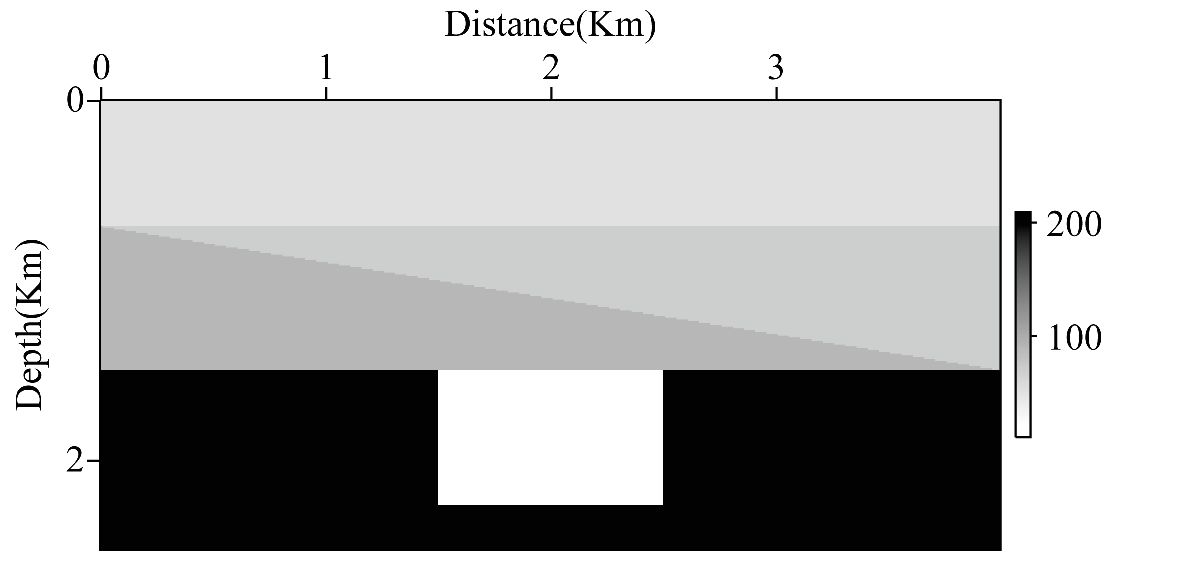
\includegraphics[width=0.82\linewidth]{figure/q_400x250}}
    \subfigure[]{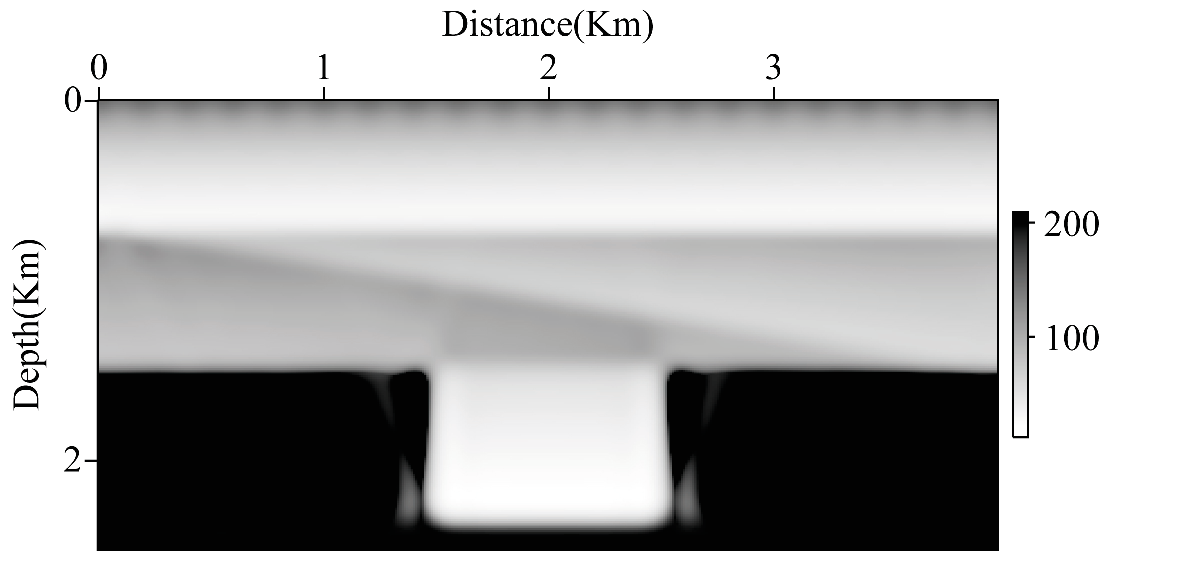
\includegraphics[width=0.82\linewidth]{figure/fq_400x250}}
    \subfigure[]{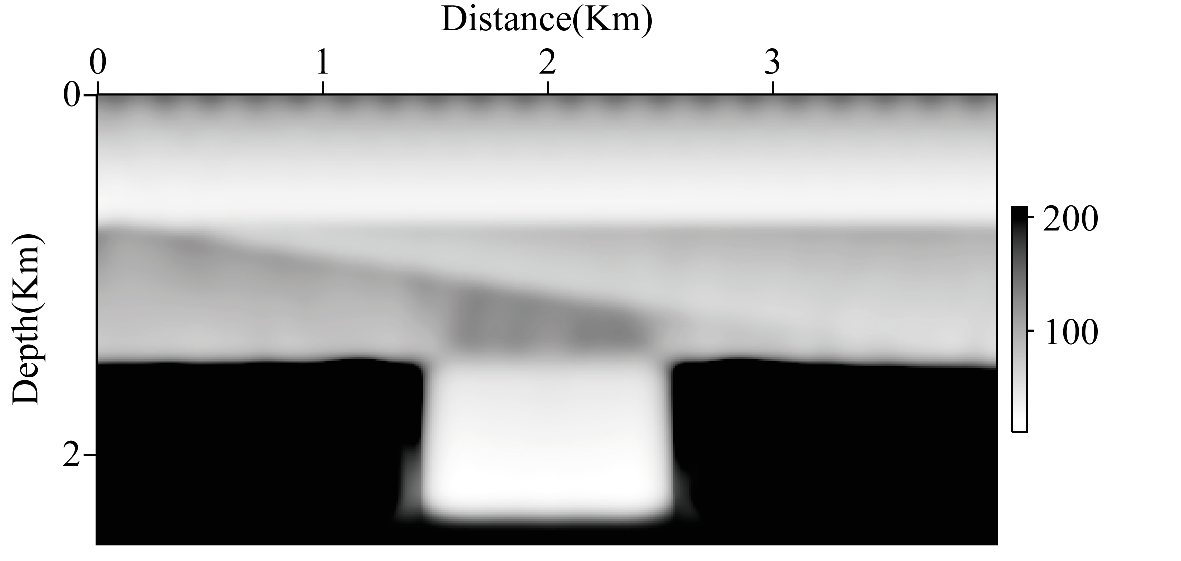
\includegraphics[width=0.82\linewidth]{figure/ffq_400x250}}
    \fcaption{层状模型反演结果:(a)真实$Q$模型;(b)基于振幅残差目标函数的
	$Q$-RWI反演结果;(c)基于峰值频率移动目标函数的$Q$-RWI
    反演结果。}{The inversion results of layered model: (a) the true $Q$ model,
    (b) inverted $Q$ model using $Q$-RWI with amplitude difference misfit function
	and (c) inverted $Q$ model using $Q$-RWI with peak frequency shift misfit function.}
    [层状模型]
    \label{fig:lens_fmodel}
\end{figure*}

\begin{figure*}[!htbp]
    \centering
    \subfigure[]{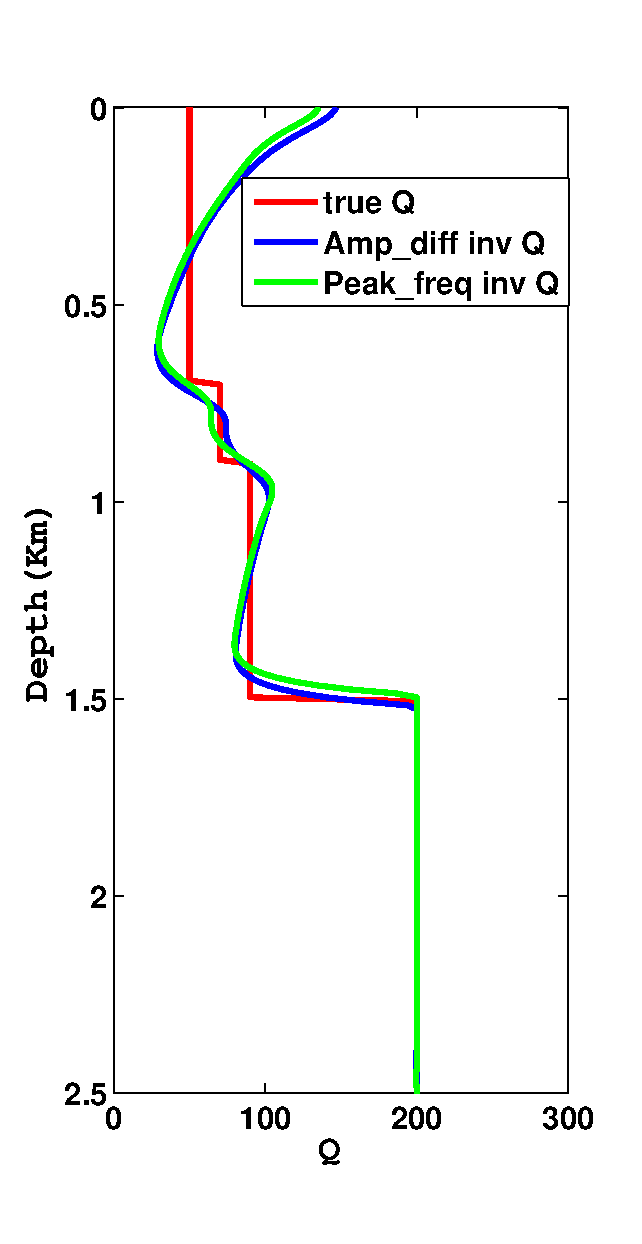
\includegraphics[width=0.32\linewidth]{figure/1km_1}}
    \subfigure[]{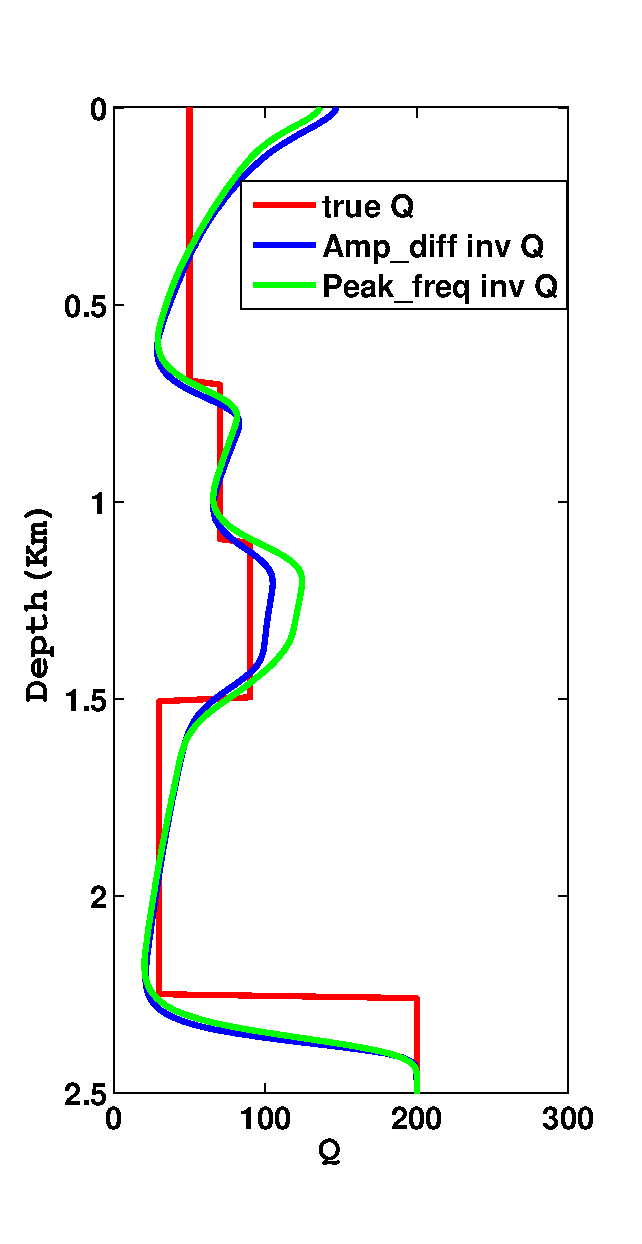
\includegraphics[width=0.32\linewidth]{figure/2km_1}}
    \subfigure[]{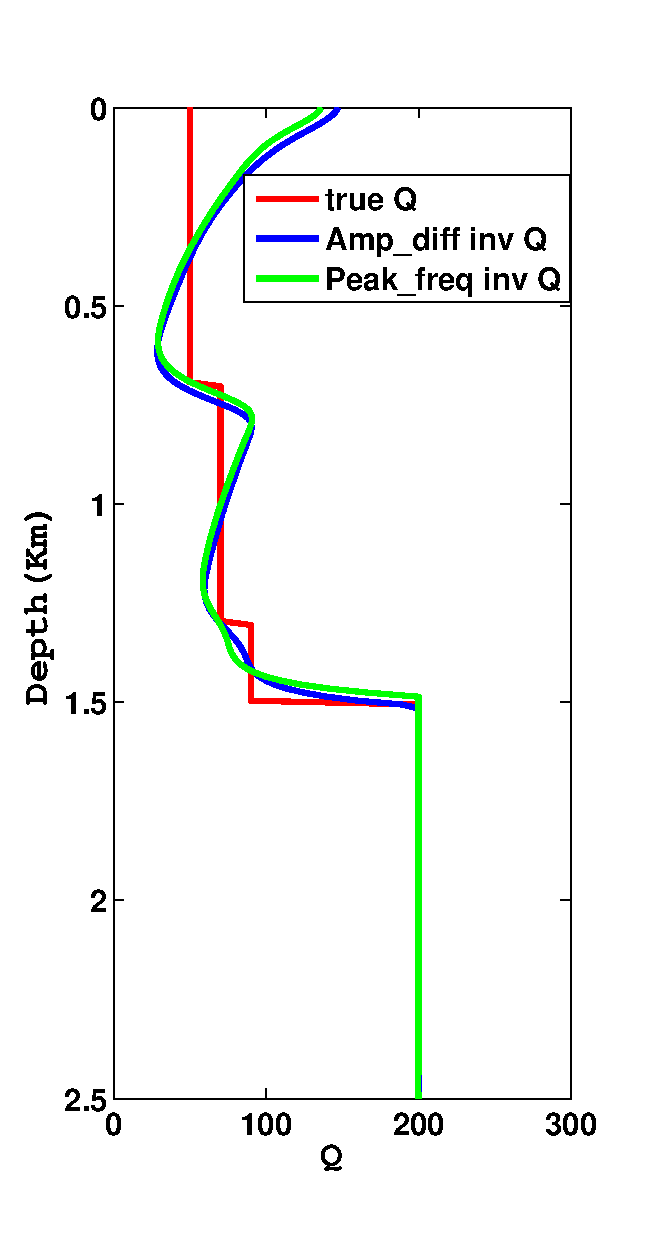
\includegraphics[width=0.32\linewidth]{figure/3km_1}}
    \fcaption{抽线对比:(a)1km处;(b)2km处;(c)3km处。其中红线是真实
	$Q$模型,蓝线是基于振幅残差目标函数的反演结果,绿线是基于峰值频率移动目标函数
	的反演结果}{Pseudowells comparison at (a) 1km, (b) 2km
    and (c) 3km. The red, blue, and green curves represent the true $Q$ model,
	amplitude difference based $Q$-RWI inversion result and peak frequency shift 
	based $Q$-RWI inversion result, respectively.}[抽线对比结果]
    \label{fig:fchouxian}
\end{figure*}

\begin{figure*}[!htbp]
    \centering
    {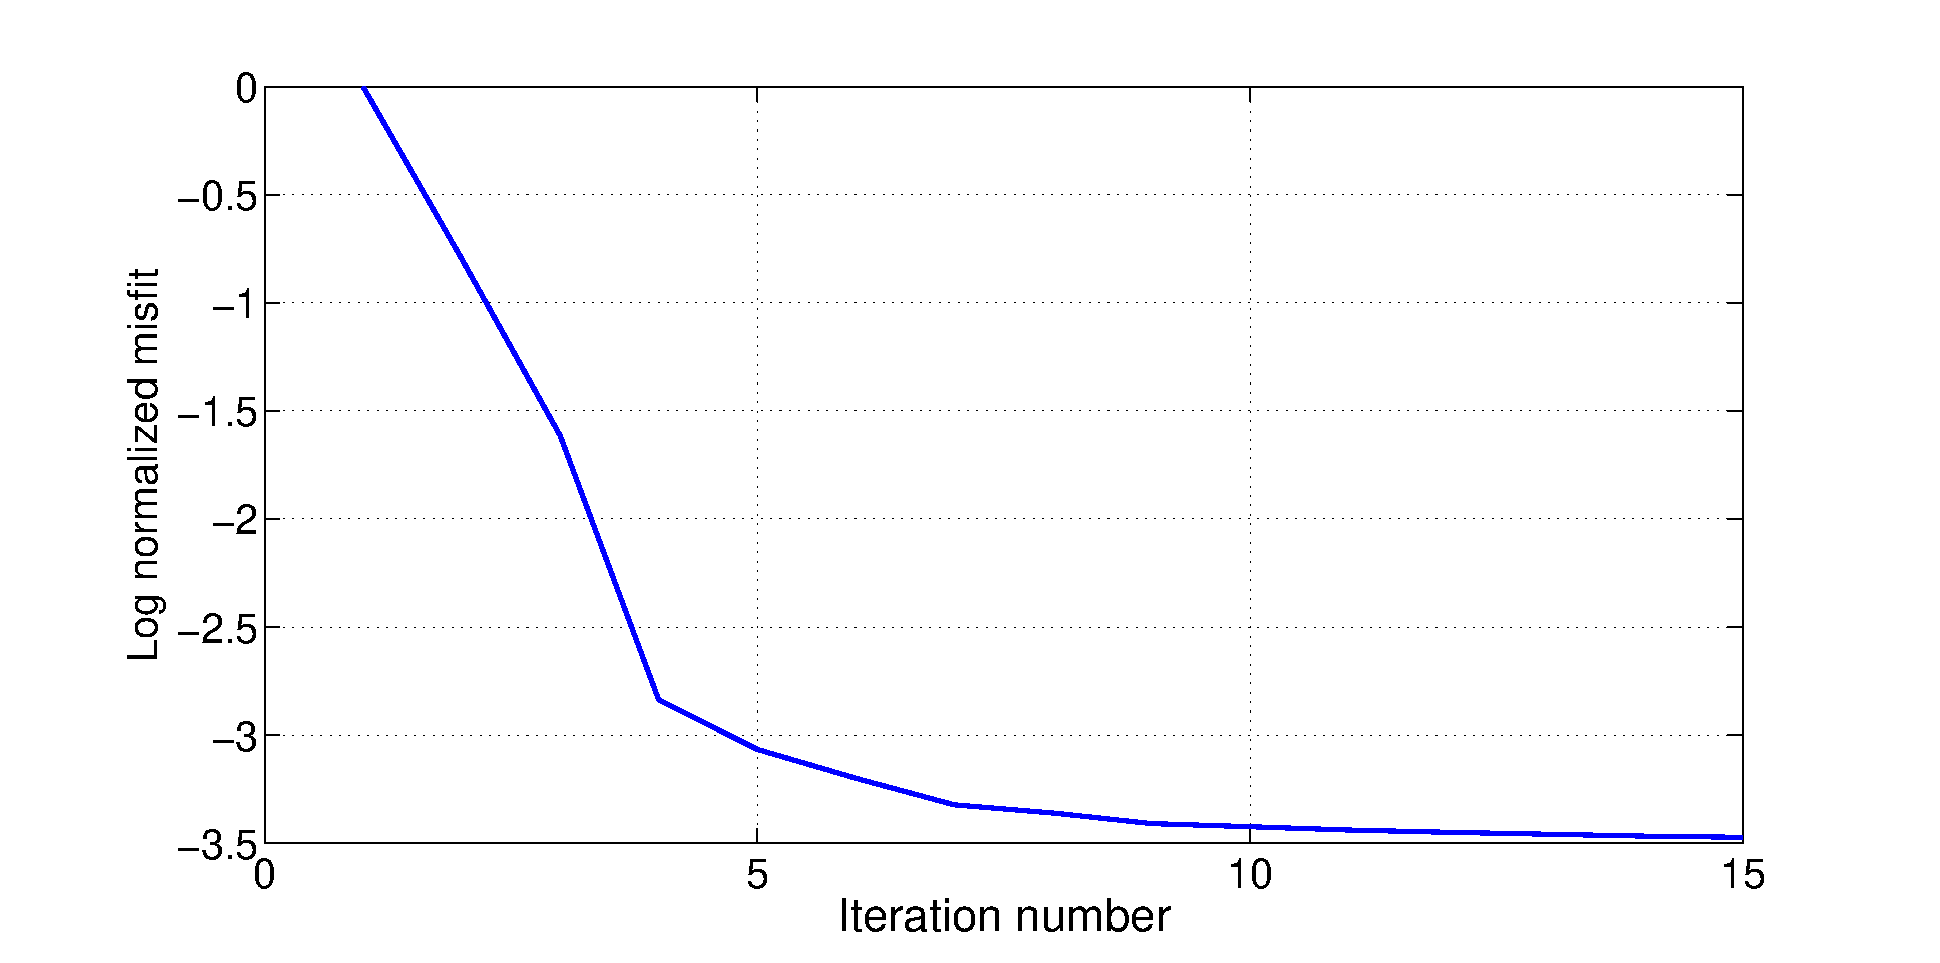
\includegraphics[width=1.0\linewidth]{figure/fmisfit}}
    \fcaption{收敛曲线}{The history of convergence.}[收敛曲线]
    \label{fig:misfit_fmodel}
\end{figure*}

\begin{figure*}[!htbp]
    \centering
    \subfigure[]{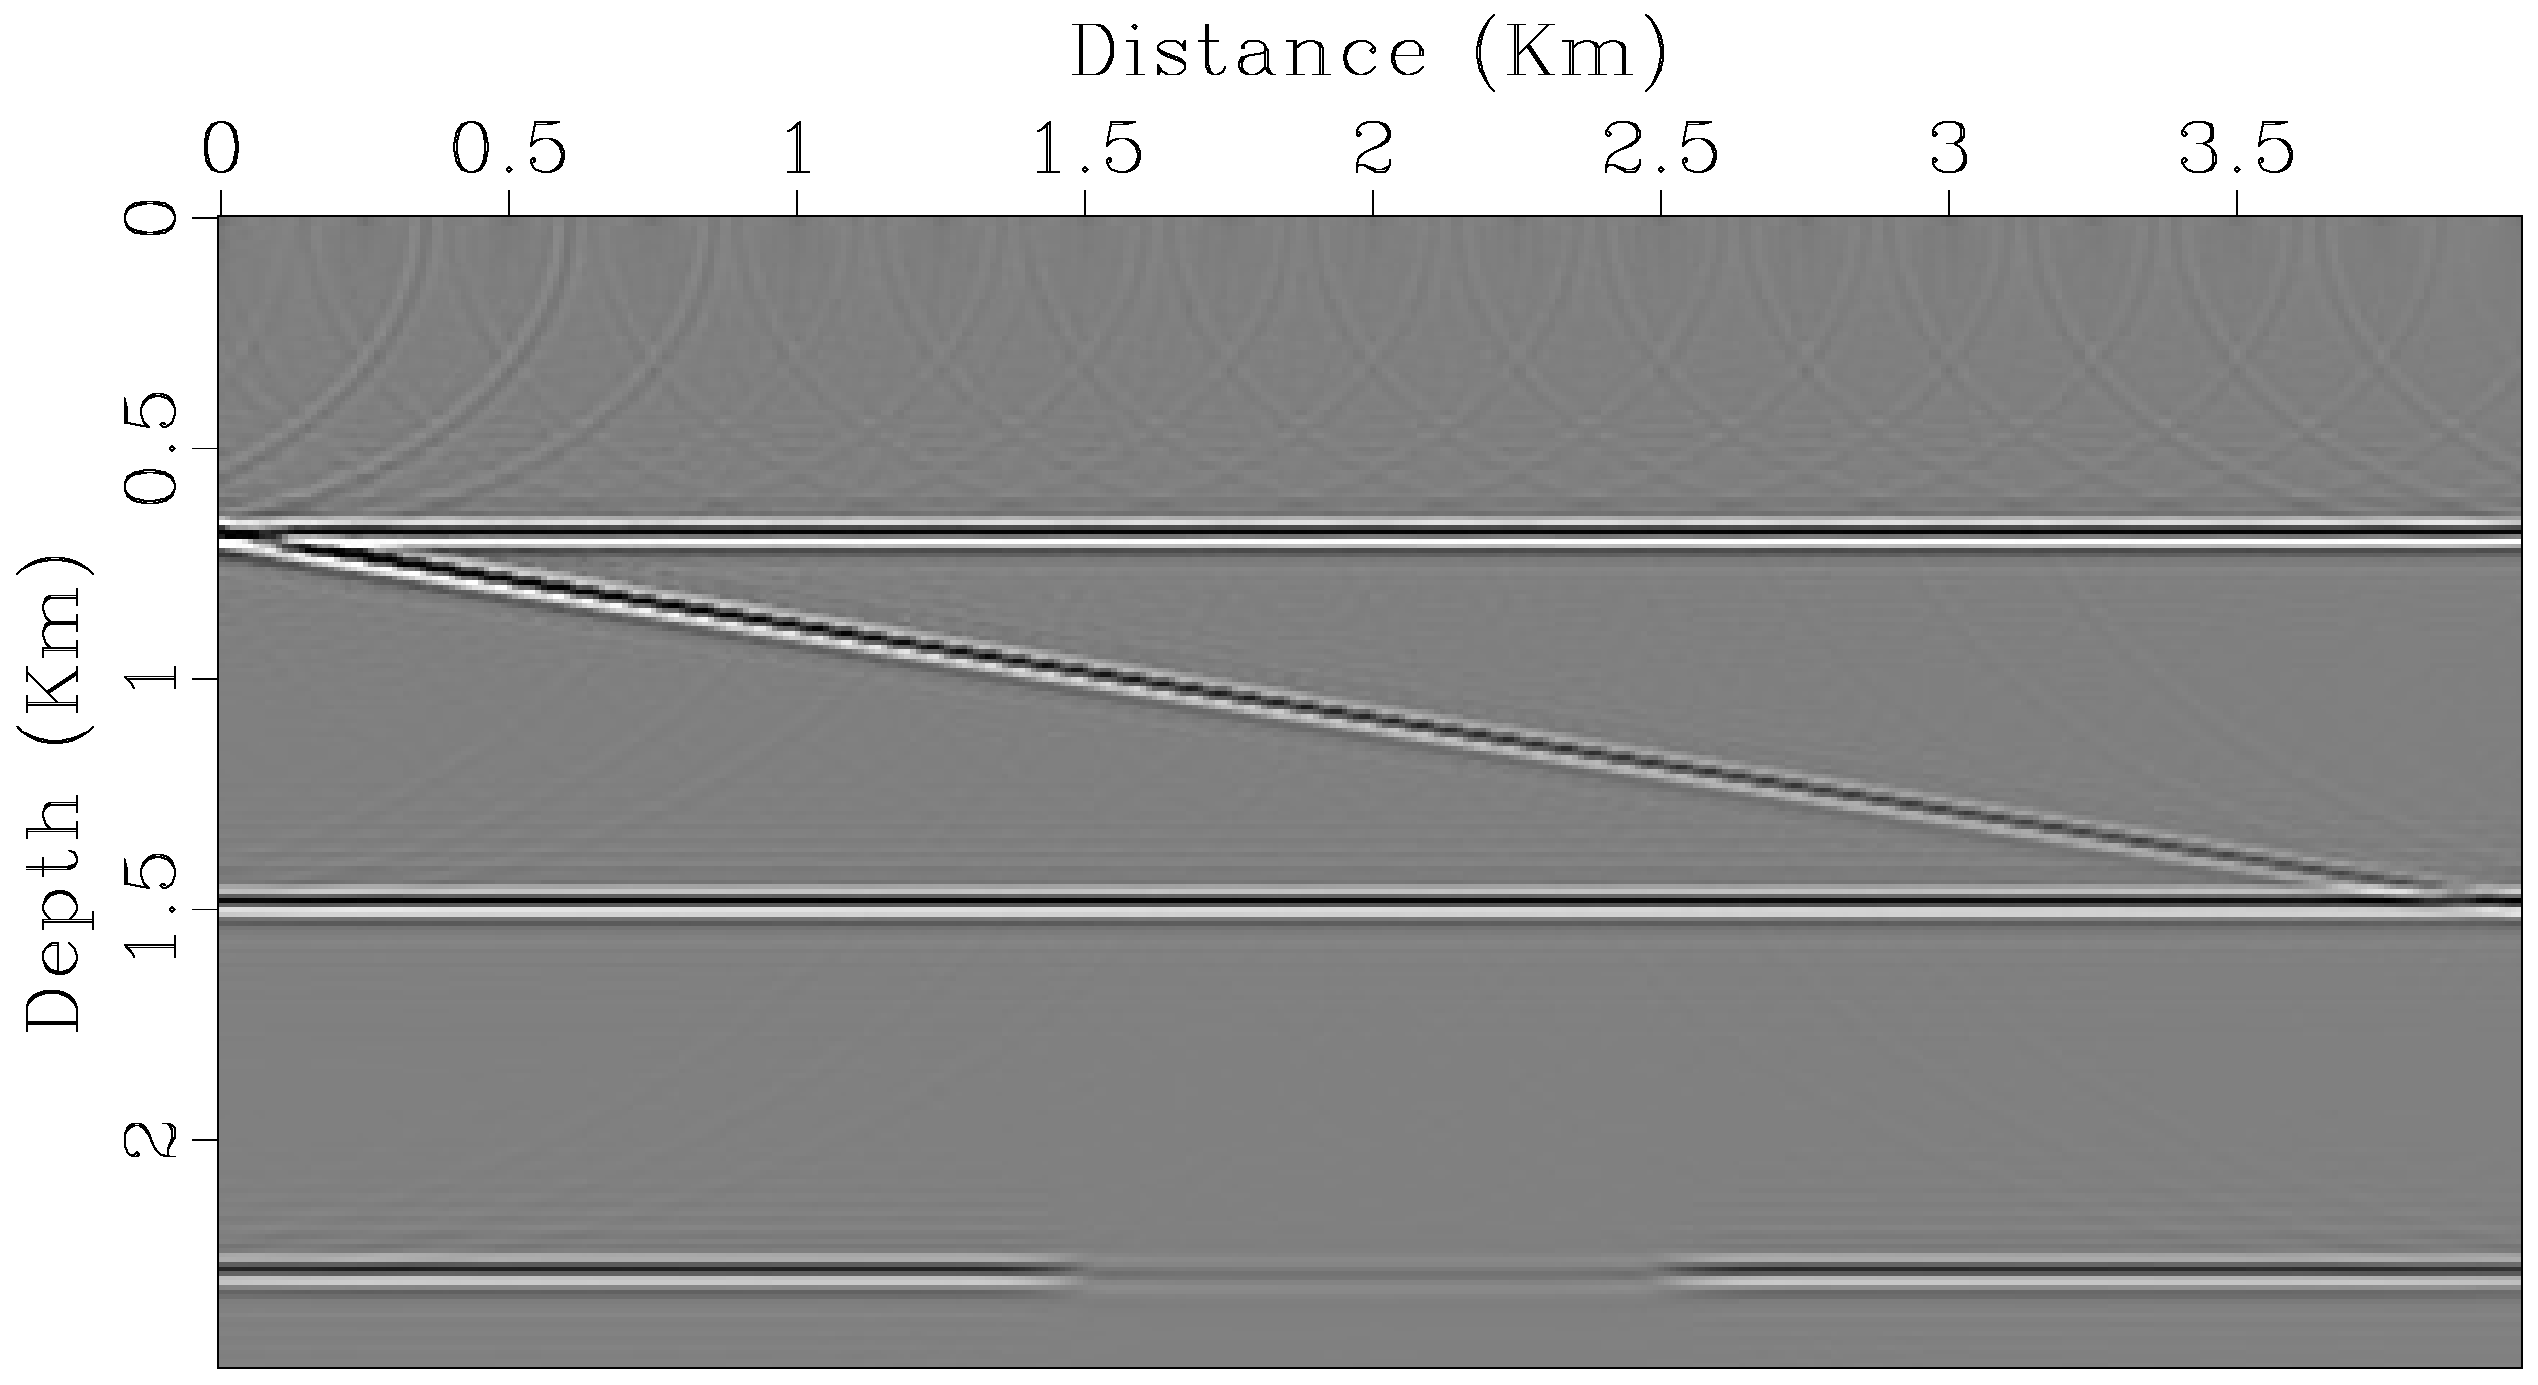
\includegraphics[width=0.72\linewidth]{figure/rtm_no400x250}}
    \subfigure[]{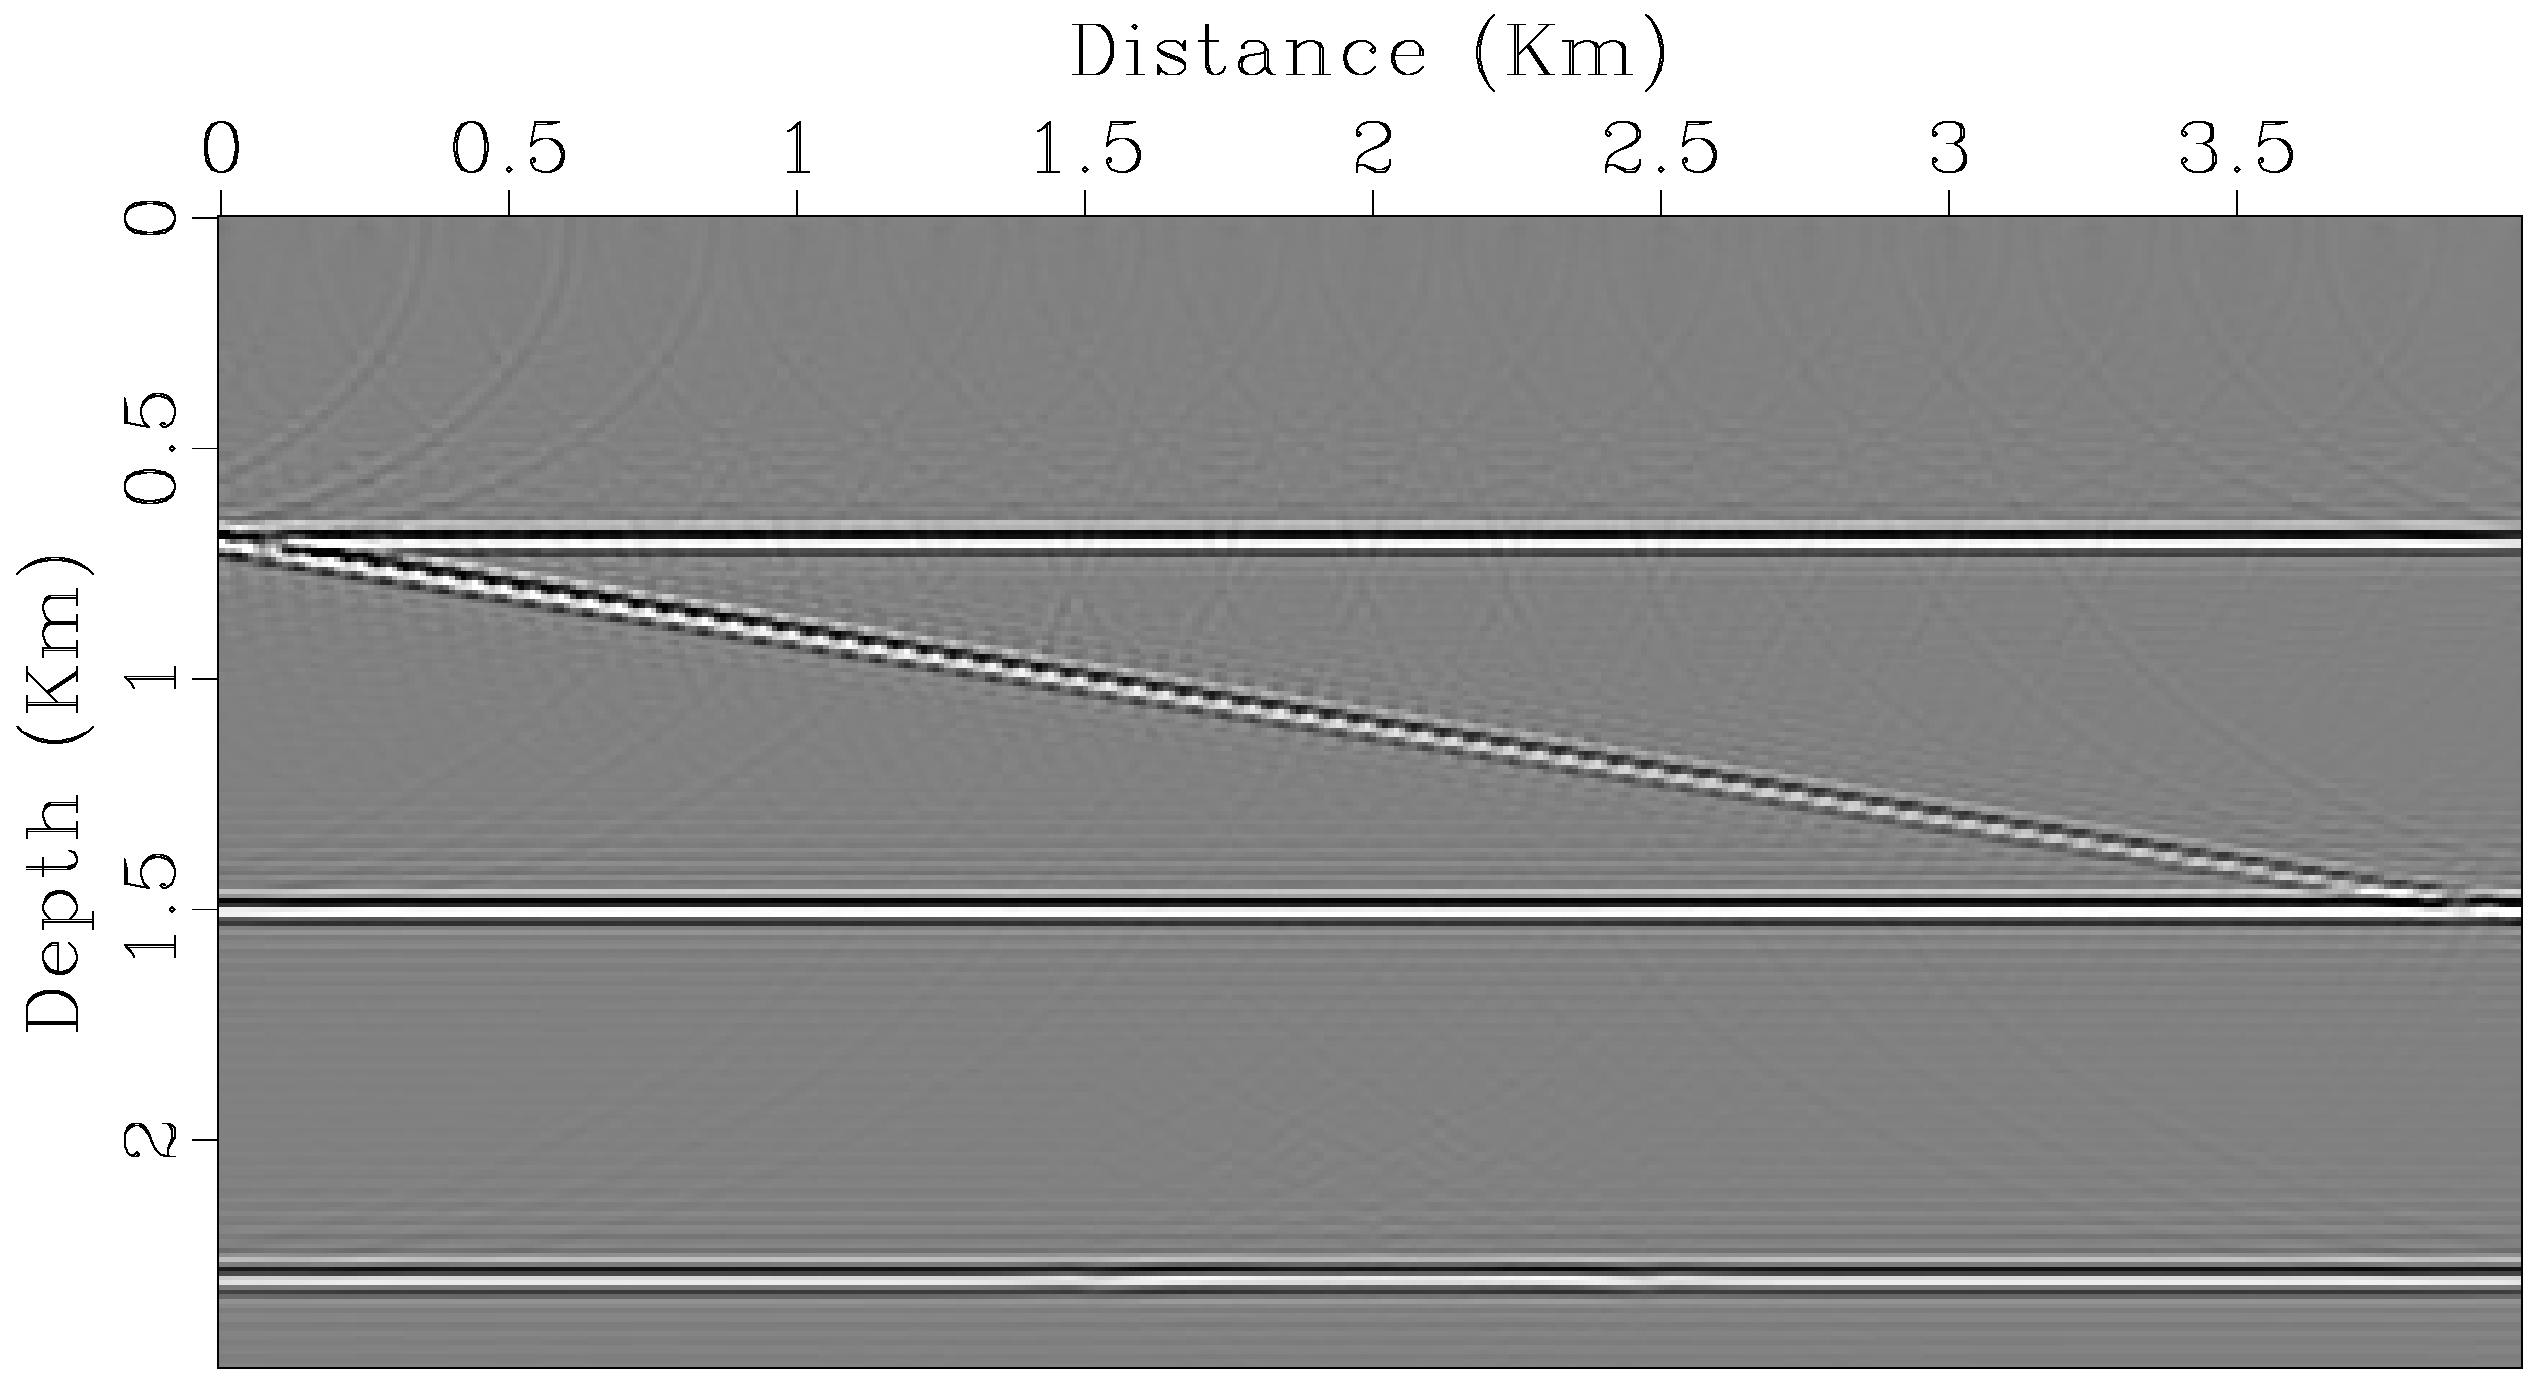
\includegraphics[width=0.72\linewidth]{figure/rtm_ffq400x250}}
    \subfigure[]{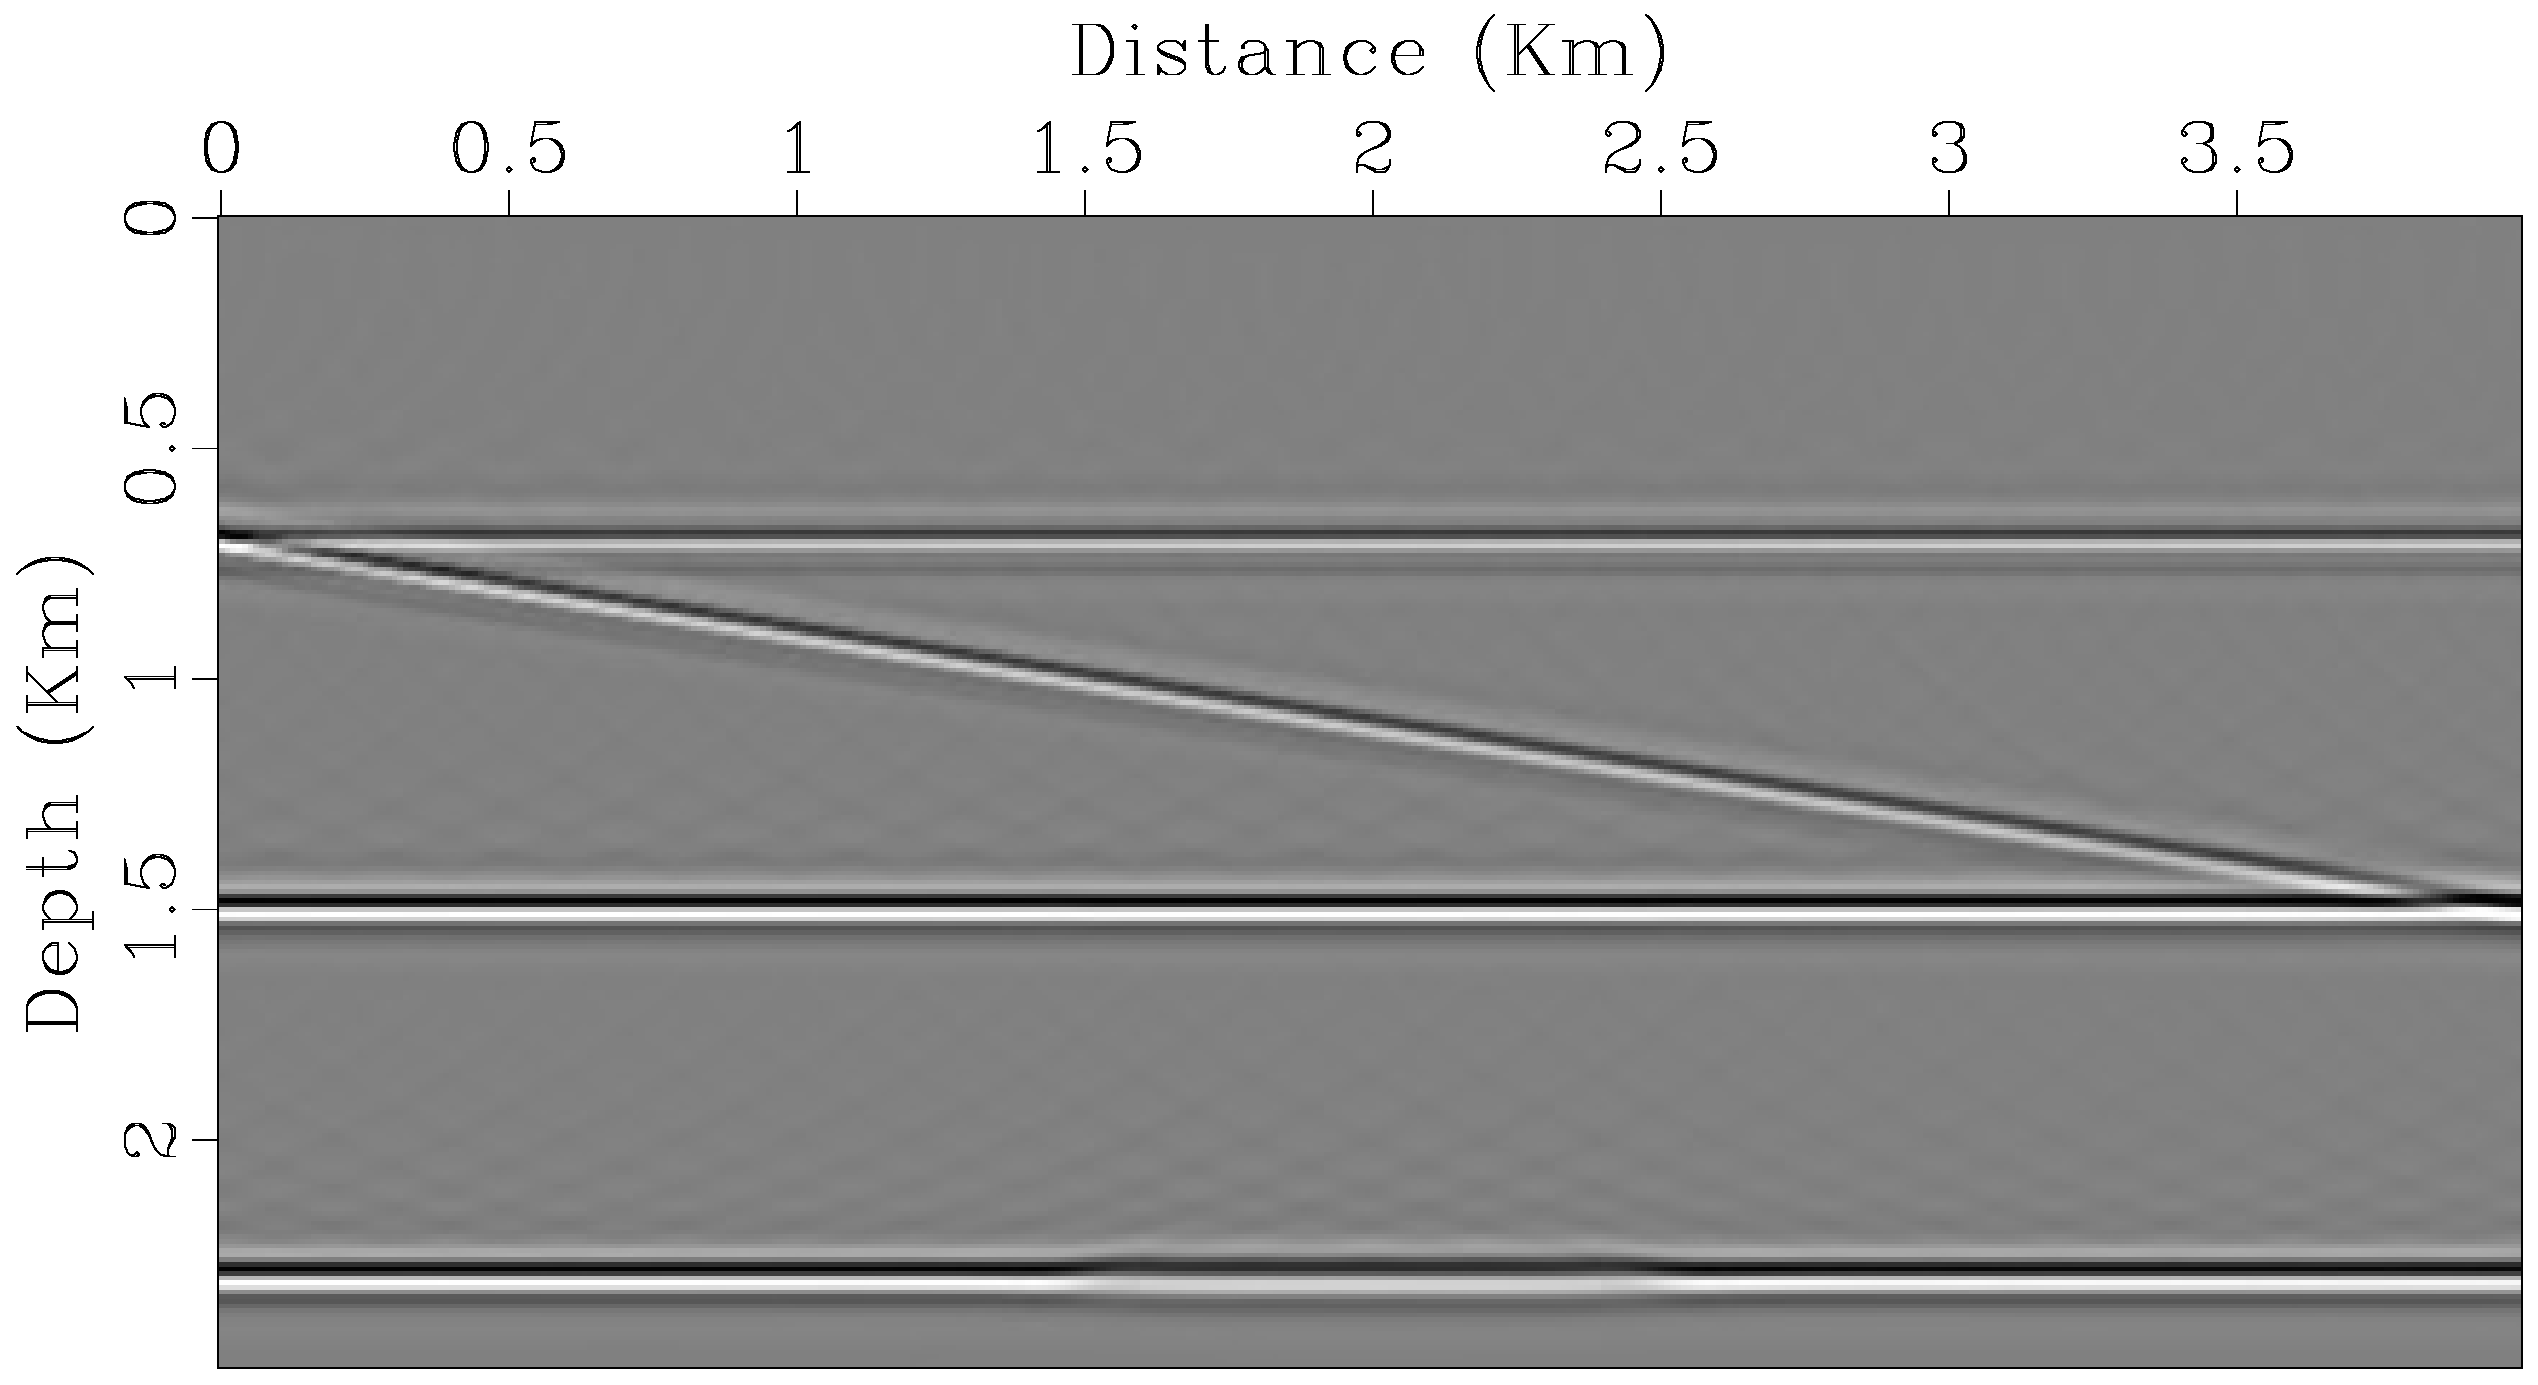
\includegraphics[width=0.72\linewidth]{figure/lsrtm_ffq400x250}}
    \fcaption{$Q$补偿成像结果:(a)初始$Q$补偿RTM结果;(b)基于峰值频率移动目标函数
    $Q$-RWI反演$Q$补偿RTM结果;(c)基于峰值频率移动目标函数$Q$-RWI反演$Q$补偿 LSRTM结果。}
	{$Q$-compensated RTM images using initial
	$Q$ model (a) and peak frequency shift based $Q$-RWI inverted $Q$ model (b); (c) is 
	$Q$-LSRTM image using the peak frequency shift based $Q$-RWI inverted $Q$ model.}
    [$Q$补偿成像结果]
    \label{fig:rtm_fmodel}
\end{figure*}

